% !TeX spellcheck = pt_BR
\documentclass[
        %oneside,         	 %%retire % do in\'icio desta linha para n\~ao imprimir frente e verso 
        english,			
%	french,				
%	spanish, 
        brazil			        %% Idioma principal 
        ,<...>]{abntbibufjf}

\usepackage{lmodern}						
\usepackage[T1]{fontenc}		
\usepackage[utf8]{inputenc}		%% Para converter automaticamente acentos como digitados normalmente no teclado. Mude utf8 para latin1 se precisar. 
\usepackage{lastpage}			
\usepackage{indentfirst}		
\usepackage{color}			
\usepackage{graphicx}			
\usepackage{microtype} 
\usepackage[portuguese,ruled,lined]{algorithm2e}
\hyphenation{Con-si-de-ra-mos}
\hyphenation{me-lhor}
\hyphenation{res-pos-ta}
\hyphenation{re-qui-si-tos}
\hyphenation{Visua-lization}
\hyphenation{Wise-Arterial-Tree}
\hyphenation{Graphic-Ob-je-ct-Factories}
\hyphenation{admi-tân-cia}
\hyphenation{vis-co-elas-ti-ci-da-de}
\hyphenation{con-si-de-ra-do}
\hyphenation{in-de-pen-den-te-men-te}
\hyphenation{fun-ci-o-na-men-to}
\hyphenation{su-ces-si-va-men-te}
\hyphenation{com-pu-ta-ci-o-nal}
\hyphenation{geo-mé-tri-cas}

%\usepackage[portuguese]{babel}  
\usepackage{listings}
\usepackage[alf,bibjustif]{abntex2cite}
\usepackage{amsmath}
\usepackage{breqn}
\usepackage{lipsum}
\usepackage{appendix}
\usepackage{multirow}

%% -----------------------------------------------------------------------------

%% Obs.: Alguns acentos foram omitidos.

\titulo{Uma Ferramenta Computacional para Simulação de Escoamento Pulsátil em Modelos de Árvores Arteriais 1D} %% Colocar, dentro de chaves {}, o t\'itulo do trabalho. Retirar % do inicio da linha seguinte se tiver subtitulo
%\subtitulo{subt\'itulo}  %% Retirar % do in\'icio desta linha se tiver subt\'itulo 
\autor{Igor Pires dos Santos} %%Colocar, dentro de chaves {}, o nome completo do autor
\autorR{Pires dos Santos, Igor} %%Colocar o sobrenome do autor, separado por v\'rgula, antes do restante do nome do autor. Ex.: Santos, Maria dos
\local{Juiz de Fora} %%Governador Valadares
\data{2021} %%Colocar o ano da entrega. Por exemplo, 2019
\orientador[Orientador:]{Rafael Alves Bonfim de Queiroz} %%Se precisar, troque [Orientador:] por [Orientadora:]
\coorientador[Coorientador:]{Ruy Freitas Reis} %% Colocar ``%'' no in\'icio desta linha se n\~ao tiver coorientador. Se precisar, troque por [Cooorientadora:]. 
\orientadorTitulo{Titula\c{c}\~ao} %%Colocar, dentro de chaves {}, a titula\c{c}\~ao do(a) orientador(a). Por exemplo, Prof. Dr.
\coorientadorTitulo{Titula\c{c}\~ao} %%Colocar, dentro de chaves {}, a titula\c{c}\~ao do(a) cooorientador(a). 
\instituicao{Universidade Federal de Juiz de Fora}
\faculdade{Programa de Pós-Graduação em Modelagem Computacional} %%Colocar, dentro de chaves {}, o nome da faculdade ou do instituto.
%\programa{Modelagem Computacional} %%Colocar, dentro de chaves {}, o nome do curso. Por exemplo: Programa de P\'os\mbox{-Gra}dua\c{c}\~ao em Matem\'atica
\objeto{Disserta\c{c}\~ao (Mestrado)}  %%Tese (Doutorado)  %%%Trabalho de Conclus\~ao de Curso (gradua\c{c}\~ao)
\natureza{Disserta\c{c}\~ao  %%Tese 
apresentada ao \insereprograma ~da   %% %%%Trabalho de conclus\~ao de curso apresentado \'a \inserefaculdade da %%%%SUBSTITUIR \'a POR ao SE FOR INSTITUTO    
Universidade Federal de Juiz de Fora como requisito parcial \`a obten\c{c}\~ao do 
t\'itulo de Mestre em  %%Doutor em    %%%grau de bacharel em 
Modelagem Computacional. %%Trocar Matem\'atica por outro, se precisar.
%\'Area de concentra\c{c}\~ao: %%PREENCHER   %%%N\~ao usar esta linha se for trabalho de conclus\~ao de curso da gradua\c{c}\~ao
}

%% Abaixo, prencher com os dados da parte final da ficha catalografica
\finalcatalog{1. Árvores arteriais. 2. Escoamento pulsátil. 3. Hemodinâmica Computacional. I. Alves Bonfim de Queiroz, Rafael, orient. II. Dr..} %% Aqui fica 
% escrito a palavra ``T\'itulo'' mesmo, nao o do trabalho. Se tiver coorientador, os dados ficam depois dos dados 
%% do orientador (II. Sobrenome, Nome do coorientador, coorient.) e antes de ``II. T\'itulo'', o qual passa a ``III. T\'itulo''.


%%Use o comando abaixo (retirando % de %\sistautordata) apenas se for usar o sistema autor-data (n\~ao o num\'erico) para refer\^encias.
%\sistautordata   


\begin{document}

%% ELEMENTOS PR\'E-TEXTUAIS

%% Capa
\inserecapa

%% Folha de rosto
\inserefolhaderosto

%% Ficha catalogr\'afica. AO IMPRIMIR, DEIXAR NO VERSO DA FOLHA DE ROSTO.
\inserecatalog  


%% Folha de aprovacao
\begin{folhadeaprovacao}
\inicfolhaaprov
        
Aprovada em (dia) de (m\^es) de (ano) %%Preencher com a data 
   
\vfill
\begin{center} BANCA EXAMINADORA \end{center}
\assinatura{\insereorientadorTitulo~\insereorientador \ - Orientador \\ Universidade Federal de Juiz de Fora}  %%Orientadora
%\assinatura{Professor Dr. \inserecoorientador \ - Coorientador \\ Universidade Federal de Juiz de Fora}
\assinatura{Titula\c{c}\~ao Nome e sobrenome \\ Universidade ???}
\assinatura{Titula\c{c}\~ao Nome e sobrenome  \\ Universidade ??} 
%\assinatura{...} %%RETIRE O % E PREENCHA SE PRECISAR
%  \assinatura{...}
%  \assinatura{...}
\end{folhadeaprovacao}
\cleardoublepage 


%% Dedicatoria. OPCIONAL. Colocar ``%'' no in\'icio de cada das 3 linhas abaixo, caso n\~ao queira.
 \begin{dedicatoria} 
  Dedico este trabalho ... 
 \end{dedicatoria}

 
%% Agradecimentos. OPCIONAL. CASO SEJA BOLSISTA, INSERIR OS DEVIDOS AGRADECIMENTOS.
\begin{agradecimentos}
Agrade\c{c}o aos ... 
\end{agradecimentos}


%% Ep\'igrafe. OPCIONAL
\begin{epigrafe} 
XXXXXXXXXXXXXXXXXXXXXX
\end{epigrafe}


%% RESUMOS

%% Resumo em Portugu\^es. OBRIGAT\'ORIO.
\begin{resumo}
\textcolor{red}{IGOR: faltar iniciar este resumo com uma introdução e motivação que podem ser tirados do seu capítulo introdução.}
Neste trabalho, apresentam-se: (i) modelo matemático da literatura que descreve o escoamento sanguíneo pulsátil em modelos de árvores arteriais 1D, (ii) uma ferramenta computacional desenvolvida que calcula a pressão e fluxo em cada vaso a partir do modelo matemático . Os resultados obtidos neste trabalho estão condizentes com dados numéricos relatados na literatura. \\[18pt]
Palavras-chave: Árvores arteriais. Escoamento pulsátil. Hemodinâmica Computacional. %finalizadas por ponto e inicializadas por letra maiuscula.
\end{resumo}
 
 
%% Resumo em Ingl\^es
\begin{resumo}[ABSTRACT]
 \begin{otherlanguage*}{english}
\textcolor{red}{IGOR: escrever primeiro o resumo em português e depois traduzi-lo.}
In this work, the following are presented: (i) an analytical scheme based on physisc and mathematic laws to calculate the local charactheristics of the pressure and flux wave in 1D arterial tree's models, (ii) a computational environment desenvolved to simulate and visualize the results of the model's construction and hemodynamic studies. The results produced in this work are consistent to real morphometric data and numeric data related in the literature. \\[18pt]
Keywords: Árvores arteriais. Pulsatile flow. Computational hemodynamics. %finalizadas por ponto e inicializadas por letra maiuscula.
 \end{otherlanguage*}
\end{resumo}

%% Seguindo o mesmo modelo acima, pode-se inserir resumos em outras l\'inguas. 


%% Lista de ilustra\c{c}\~oes. OPCIONAL. 
\pdfbookmark[0]{\listfigurename}{lof}  

%Caso as ilustra\c{c}~oes do trabalho sejam todas do mesmo tipo (por exemplo, todas do tipo organograma), coloque % no in\\'icio das duas linhas abaixo. 
\ilustvaria   %Use este comando somente caso as ilustra\c{c}\~oes n\~ao sejam todas do mesmo tipo. 
\listilustvaria  %Use este comando somente caso as ilustra\c{c}\~oes n\~ao sejam todas do mesmo tipo e caso queira inserir a lista delas. 

%\listoffigures*  %Use este comando quando todas as ilustra\c{c}\~oes s\~ao do mesmo tipo e caso queira inserir a lista delas. Veja dicas no final deste arquivo.

\cleardoublepage
%% Lista de tabelas. OPCIONAL. 
\pdfbookmark[0]{\listtablename}{lot}
\listoftables*    %Coloque ``%'' no in\'icio desta linha, caso n\~ao queira lista de tabelas.
\cleardoublepage


%% Lista de abreviaturas e siglas. OPCIONAL
%\begin{siglas} %%ALTERAR OS EXEMPLOS ABAIXO, CONFORME A NECESSIDADE
%  \item[ABNT] Associa\c{c}\~ao Brasileira de Normas T\'ecnicas
%  \item[Fil.] Filosofia
%  \item[IBGE] Instituto Brasileiro de Geografia e Estat\'istica
%  \item[INMETRO] Instituto Nacional de Metrologia, Normaliza\c{c}\~ao e Qualidade Industrial
%\end{siglas}

%% Lista de s\'imbolos. OPCIONAL
\begin{simbolos} 
\item [$p$] Pressão
\item [$q$] Fluxo
\item [$t$] Tempo
\item [$x$] Coordenada axial ao longo do tubo arterial
\item [$c$] Velocidade de onda
\item [$Y$] Admitância do segmento arterial
\item [$Y_r$] Valor da admitância característica do vaso raiz
\item [$A$] Área da seção transversal do vaso
\item [$\rho$] Densidade do fluido
\item [$w$] Frequência angular
\item [$f$] Frequência da onda
\item [$L$] Comprimento do tubo arterial
\item [$k$] Geração do vaso na árvore
\item [$j$] Posição do vaso na geração da árvore
\item [$E$] Módulo de Young
\item [$h$] Espessura da parede do vaso
\item [$p_f$] Pressão na posição proximal do vaso
\item [$p_b$] Pressão na posição distal do vaso
\item [$R$] Coeficiente de Reflexão
\item [$Y_e$] Admitância efetiva do vaso
\item [$\alpha$] Número de Womersley
\item [$\epsilon$] Fator viscoso do vaso
\item [$\phi$] Propriedade  atrelada a viscoelasticidade da parede
\item [$\mu$] Viscosidade no segmento arterial
\item [$J_p$] Função de Bessel de índice $p$
 \end{simbolos}

 
%% Sum\'ario
\pdfbookmark[0]{\contentsname}{toc}
\tableofcontents*
\cleardoublepage

%% ----------------------------------------------------------

%% ELEMENTOS TEXTUAIS
\textual


%--------------------------------------------------------------------------------%
\chapter{INTRODUÇÃO}\label{sec:intro}  %%Nesta linha, dentro de { }, digita-se em CAIXA ALTA, como apresentado aqui

Estudos de simulação hemodinâmica têm sido frequentemente baseados em modelos de árvores arteriais para obter uma melhor compreensão de todos os aspectos relacionados ao escoamento sanguíneo, desde a propagação de ondas e análise do pulso de pressão, passando pelo diagnóstico e inclusive com aplicações no planejamento cirúrgico. Como a representação do sistema cardiovascular através de um modelo puramente 3D que leve em conta a estrutura geométrica exata de todos os vasos não é, no momento, viável computacionalmente, vêm sendo empregados modelos dimensionalmente heterogêneos conhecidos como 0D (zero-dimensional)--1D (unidimensional)--3D (tridimensional) \cite{Formaggia2001}. 

Modelos 3D \cite{Peskin1972,Taylor1998} são utilizados para estudar em detalhe a hemodinâmica local de distritos arteriais de interesse, e a geometria destes modelos são provenientes de dados anatômicos obtidos normalmente via reconstrução de imagens médicas de pacientes específicos. Modelos 1D \cite{Avolio,Formaggia2003,Stergiopulos1992} são adotados para representar as artérias de maior calibre e a estrutura geométrica destes modelos pode ser construída a partir de dados anatômicos. Tais modelos são capazes de capturar os efeitos de propagação de ondas~\cite{Anliker1971,Duan}, a interação das reflexões destas ondas e dar como resultado um pulso de pressão e vazão com significado fisiológico tanto em artérias centrais como periféricas. No entanto, um modelo 1D de toda a árvore arterial sistêmica não é possível devido à falta de dados anatômicos precisos das regiões periféricas. Portanto, a árvore tem que ser truncada em algum nível. Normalmente, este truncamento é feito empregando modelos 0D \cite{Mates1988,Stergiopulos1992} conhecidos por terminais Windkessel à jusante da posição distal do modelo 1D para representar o comportamento de distritos arteriais relacionados com o nível de arteríolas e capilares. 

\textcolor{red}{IGOR: os dois parágrafos acima estão legais no sentido da ideia para se colocar em uma introdução, mais necessitam ser um pouco reescritos e principalmente, citar referências mais recentes de estudos hemodinâmicas envolvendo modelos 3D, 1D, 0D, e modelos acoplados 0D-1D, 3D-1D-0D. Vale a pena buscar estas referências e ler a introdução deste artigos}

A incidência maior de picos na onda de pressão ao percorrer a aorta já foi documentada como evidência para os efeitos da reflexão em árvores vasculares \cite{Kouchoukos,Lighthill,McDonald}. Enquanto as áreas de reflexão não podem ser completamente conhecidas ou localizadas, é geralmente aceito que a forma da onda de pressão é modificada significativamente enquanto progride pela aorta, de uma forma que só pode ser explicada por reflexões de onda.  Um entendimento mais claro da relação entre modificações e fatores de modificação motiva a busca e desenvolvimento de modelos matemáticos que determinam a forma da onda que o pulso de pressão toma em cada ponto ao percorrer uma árvore arterial. 

Dentro deste contexto, adotou-se neste trabalho o modelo matemático de Duan e Zamir ~\cite{Duan} que descreve escoamento sanguíneo pulsátil em árvores arteriais. Estes autores propuseram um modelo relativamente simples para representação da pressão sanguínea e do fluxo em um modelo de árvore arterial. Dentro de cada segmento de vaso, o escoamento sanguíneo foi calculado baseado em uma aproximação de Womersley, incluindo a elasticidade da parede, bem como a densidade do sangue e a viscosidade.

A capacidade de capturar o pico de pressão existente no escoamento sanguíneo justificativa a escolha do modelo matemático de Duan e Zamir para implementação e simulação computacional. Este modelo possibilita o cálculo correto das características locais das ondas de pressão e fluxo a medida que elas progridem ao longo de um modelo de árvore 1D e se tornam modificadas por reflexões de onda.

\textcolor{red}{IGOR: escreva um parágrafo de trabalhos da literatura que citam e utilizam o modelo de Duan e Zamir. Busque referências na literatura. Lembrando que esta referência \cite{Duan} está errada. A referência correta é de 1995. Principalmente, cite o seu trabalho publicado na revista Mundi deste parágrafo.}

%--------------------------------------------------------------------------------%
\section{Objetivos}\label{sec:obj}

Os objetivos que norteiam este trabalho são:
\begin{itemize}
    \item desenvolver uma ferramenta computacional capaz de simular o modelo matemático de Duan e Zamir;
    \item aplicar a ferramenta desenvolvida considerando diferentes cenários hemodinâmicos para investigar os efeitos da viscosidade sanguínea e da viscoelasticidade da parede do vaso no escoamento sanguíneo
\end{itemize}

%--------------------------------------------------------------------------------%
\section{Organização}\label{sec:org}

Os demais capítulos deste trabalho estão organizados como segue:
\begin{itemize}
    \item Capítulo 2 -
    
    \item Capítulo 3 --
    Neste capítulo, apresenta-se a ferramenta computacional desenvolvida em C++,  a qual contou com a utilização das bibliotecas Qt/OpenGL para ajudar na elaboração da interface gráfica
    \item Capítulo 4 ---
    
    \item Capítulo 5
\end{itemize}

\textcolor{red}{IGOR: complemente esta seção de organização. Recomendo fortemente ler a introdução da minha dissertação e tese para ter mais ideias de como montar uma introdução para sua dissertação.}

%--------------------------------------------------------------------------------%
\chapter{MODELAGEM DO ESCOAMENTO SANGUÍNEO}\label{sec:modelagem_escoamento}

%\textcolor{red}{IGOR: está errada a citação do trabalho do método de Duan e Zamir (1995), não é a citação que colocou \cite{Duan}.}

Neste capítulo, apresenta-se em detalhe o modelo matemático de Duan e Zamir \cite{Duan}, para o escoamento sanguíneo pulsátil em árvores arteriais. Por fim, apresenta um algoritmo que sistematiza os passos dos cálculos realizados para obtenção da pressão e fluxo ao longo da árvore arterial.

%--------------------------------------------------------------------------------%
\section{MODELO MATEMÁTICO}\label{sec:modelo_matematico}

A propagação de ondas em um tubo é governada pela equações da onda para a pressão $p(x,t)$ e fluxo $q(x,t)$ como seguem:
\begin{eqnarray}
\frac{\partial q}{\partial t} &=& -cY \frac{\partial p}{\partial x},
\label{01_p}\\
\frac{\partial p}{\partial t} &=& -\frac{c}{Y} \frac{\partial q}{\partial x}, 
\label{02_q}
\end{eqnarray}
nos quais $t$ é o tempo, $x$ é a coordenada axial ao longo do tubo, $c$ é a velocidade de onda, $Y = \frac{A}{\rho c}$ é a admitância e $A$ é a área da seção transversal do tubo, e $\rho$ é a densidade do fluido. Estas equações são baseadas na linearização das equações de movimento do fluido \cite{Fung,Lighthill}. 

Para uma onda harmônica simples, as equações (\ref{01_p}) e (\ref{02_q}) resultam em:
\begin{eqnarray}
p &=& \bar{p}_0 \exp\left[i\omega\left(t - \frac{x}{c}\right)\right] + R  \bar{p}_0 \exp\left[i\omega\left(t - \frac{2L}{c} + \frac{x}{c}\right)\right],
\label{03_p}\\
q &=& Y\left\{\bar{p}_0 \exp\left[i\omega\left(t - \frac{x}{c}\right)\right] -  R  \bar{p}_0 \exp\left[i\omega\left(t - \frac{2L}{c} + \frac{x}{c}\right)\right]\right\},
\label{04_1}
\end{eqnarray}
onde $\omega = 2 \pi f$ é a frequência angular, $f$ é frequência em Hertz, $L$ é o comprimento do tubo, $\bar{p}_0$ é a amplitude da onda incidente, $R$ é o coeficiente de reflexão definido pela razão entre as ondas refletidas pelas ondas que chegam no local de reflexão \cite{Fung,Karreman} e $i$ é a unidade imaginária ($i^2 = -1$).

As equações \eqref{03_p} e \eqref{04_1} para pressão e fluxo são aplicadas em cada segmento de vaso do modelo de árvore arterial, tomando $x = 0$ para o nó proximal e $x = L$ para o nó distal do segmento. Um segmento de vaso é definido pelo intervalo vascular entre dois locais de ramificação \cite{Zamir3}. No sistema arterial, as bifurcações são os locais de ramificação mais comuns~\cite{Zamir1}.

Em \cite{Duan}, um segmento de vaso é identificado por $(k,j)$, onde o primeiro $k$ representa o nível da geração e $j$ representa a ordem do segmento naquela geração, como mostrado na Figura \ref{fig1:arterial-tree}. Desta forma, a pressão e o fluxo ao longo de um segmento  $(k,j)$ do modelo de árvore arterial são dados por:
\begin{eqnarray}
p(k,j) &=& \bar{p}(k,j) \exp\left[i\omega\left(t - \frac{x(k,j)}{c(k,j)}\right)\right] \nonumber \\
&+& R(k,j)  \bar{p}(k,j) \exp\left[i\omega\left(t - \frac{2L(k,j)}{c(k,j)} + \frac{x(k,j)}{c(k,j)}\right)\right],
\label{05_p}\\
q (k,j) &=& Y(k,j)\left\{\bar{p}(k,j) \exp\left[i\omega\left(t - \frac{x(k,j)}{c(k,j)}\right)\right]\right. \nonumber \\
&-& \left. R(k,j)  \bar{p}(k,j) \exp\left[i\omega\left(t - \frac{2L(k,j)}{c(k,j)} + \frac{x(k,j)}{c(k,j)}\right)\right]\right\},
\label{06_q}
\end{eqnarray}
nos quais $\bar{p}(k,j)$ é a amplitude combinada do grupo de ondas progressivas no segmento $(k,j)$ e $R(k,j)$ é o coeficiente de reflexão no final daquele segmento, como é chamado a razão das ondas progressivas pelas atrasadas avaliadas no nó distal $x(k,j) = L(k,j)$. 

O grupo de ondas progressivas viaja no sentido positivo de $x(k,j)$, estas são compostas de ondas progressivas vindo de vasos acima deste, bem como, ondas refletidas na junção à montante $x(k,j) = 0$. O grupo de ondas atrasadas viaja no sentido oposto e é composto por ondas vindas de vasos à jusante como ondas refletidas na junção à jusante $x(k,j) = L(k,j)$. 

As equações \eqref{05_p} e \eqref{06_q} descrevem, respectivamente, as ondas de pressão e de fluxo localmente em um segmento $(k,j)$ do modelo de árvore, e localmente na posição $x(k,j)$ dentro deste segmento de vaso. As duas variáveis desconhecidas são a amplitude da pressão  $\bar{p} (k,j)$ e o coeficiente de reflexão $R (k,j)$, que são detalhados na Seção~\ref{sec:pressao-fluxo}. 

A Figura~\ref{fig1:arterial-tree} mostra a notação usada para identificar cada segmento de vaso $(k,j)$, onde $k$ é a geração/nível do vaso e $j$ é um número sequencial dentro daquela geração. Os nós proximal e distal do segmento $(k,j)$ são denotados por $A$ e $B$, respectivamente. O coeficiente de reflexão $R(k,j)$ do segmento $(k,j)$ está associado ao nó distal $B$.

Na equação~\eqref{06_q}, tem-se a admitância característica para cada segmento dada por:
\begin{equation}
Y(k,j) = \frac{A(k,j)}{\rho(k,j)c(k,j)},
\label{eq:admitancia}
\end{equation}
nos quais $A(k,j)$ é a área da seção transversal do segmento $(k,j)$, $\rho(k,j)$ é a densidade do fluido dentro do vaso e $c(k,j)$ é a velocidade da onda correspondente. A admitância de um segmento é uma medida do quanto o segmento permite o fluxo.

Assumindo um segmento elástico de parede fina, a velocidade da onda $c(k,j)$ é calculada
por~\cite{Fung}:
\begin{equation}
c(k,j) = \sqrt{\frac{E(k,j) h(k,j)}{\rho(k,j) d(k,j)}},\label{eq:velocidade}
\end{equation}
onde $E(k,j)$ é o módulo de Young, $d(k,j)$ é o diâmetro do segmento $(k,j)$ e $h(k,j)$ é a espessura da parede do segmento, a qual neste estudo é dada por~\cite{Duan}: 
\begin{equation}
h(k,j) = 0,05 d(k,j).
\end{equation}

\begin{figure}[h] 
	\begin{center}
		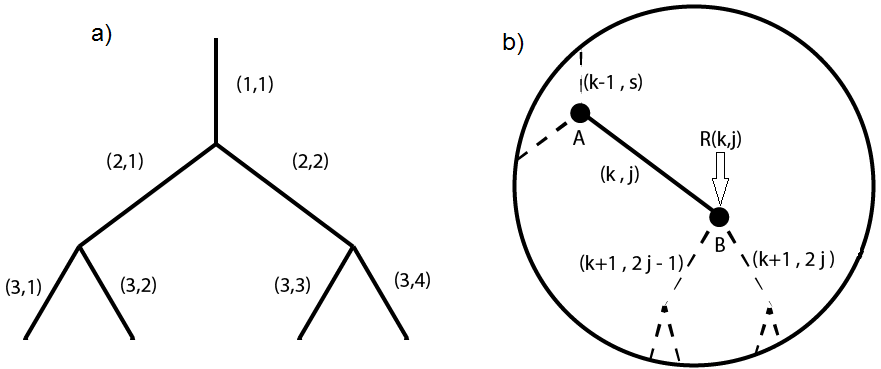
\includegraphics[scale = 0.5]{Figures/ArterialTree_Zamir.png}%
		\caption{Notação usada para identificar cada segmento de vaso $(k,j)$ (figura adaptada de~\cite{Duan}). }
		\label{fig1:arterial-tree}%
	\end{center}
\end{figure}

%--------------------------------------------------------------------------------%
\subsection{Cálculo da pressão e do fluxo sanguíneo}\label{sec:pressao-fluxo}

Para determinar a pressão $\bar{p} (k,j)$ em um certo segmento $(k,j)$, aplica-se a condição de continuidade de pressão no nó proximal $A$ (ver Figura \ref{fig1:arterial-tree}). Escrevendo as componentes progressiva e atrasada da onda como $p_f (k,j)$ e $p_b (k,j)$ respectivamente, a pressão na posição proximal do segmento  $x(k,j) = 0$ é dada por:
\begin{equation}
\left[ p (k,j) \right]_A = \left[ p_f (k,j) \right]_A + \left[ p_b (k,j)\right]_A,
\label{09_p}
\end{equation}
nos quais as pressões $\left[ p_f(k,j) \right]_A$ e $\left[ p_b(k,j) \right]_A$ são expressas por:
\begin{eqnarray}
\left[ p_f(k,j) \right]_A &=& \bar{p}(k,j)\exp\left[ i\omega t\right],
\label{10_p_f}\\
\left[ p_b (k,j) \right]_A &=& R(k,j)\bar{p}(k,j)\exp\left[i\omega \left(t - \frac{2L(k,j)}{c(k,j)}\right) \right].
\label{11_p_b}
\end{eqnarray}
Similarmente, a pressão no segmento pai $(k-1,s)$ pode ser escrita como:
\begin{equation}
p(k-1,s) =  p_f(k-1,s) + p_b (k-1,s),
\label{12_p|_f}
\end{equation}
nos quais $s$ é um número sequencial do segmento pai e as pressões $ p_f (k-1,s)$ e $p_b (k-1,s)$ são dadas por:
\begin{eqnarray}
p_f (k-1,s) &=& \bar{p}(k-1,s)\exp\left[i\omega \left(t - \frac{x(k-1,s)}{c (k-1,s)}\right) \right],\\
\label{13_p_f}
p_b (k-1,s) &=& R (k-1,s)\bar{p}(k-1,s)\exp\left[ i\omega \left( t - \frac{2L(k-1,s)}{c(k-1,s)} + \frac{x(k-1,s)}{c(k-1,s)}\right) \right]. \nonumber
\end{eqnarray}

No nó distal do vaso superior, $x(k-1,s) = L(k-1,s)$, a pressão é dada por:
\begin{equation}
\left[ p(k-1,s) \right]_A = \left[ p_f(k-1,s)\right]_A + \left[ p_b(k-1,s) \right]_A,
\label{13_p|_f}
\end{equation}
nos quais 
\begin{eqnarray}
\left[ p_f(k-1,s) \right]_A &=& \bar{p}(k-1,s)\exp\left[ i\omega \left(t - \frac{L(k-1,s)}{c(k-1,s)}\right)\right],
\label{15_p_f}
\\
\left[ p_b(k-1,s) \right]_A &=& R(k-1,s)\bar{p}(k-1,s)\exp\left[i\omega \left( t - \frac{L(k-1,s)}{c(k-1,s)} \right) \right]. 
\label{16_p_b}
\end{eqnarray}

A condição de continuidade da pressão exige que na junção ela assuma um único valor, portanto
\begin{equation}
\left[ p_f(k-1,s) \right]_A + \left[ p_b (k-1,s) \right]_A = \left[ p_f(k,j) \right]_A + \left[ p_b(k,j) \right]_A.
\label{17_p_cont}
\end{equation}

Substituindo as equações \eqref{10_p_f}, \eqref{11_p_b}, \eqref{15_p_f} e \eqref{16_p_b} na equação \eqref{17_p_cont} e resolvendo para $\bar{p}(k,j)$, resulta em:
\begin{equation}
\bar{p} (k,s) =  \frac{\bar{p}(k-1,s)\left[1 + R(k-1,s)\right] \exp\left[ -\frac{i \omega L(k-1,s)}{c(k-1,s)}\right]}{1 + R(k,j)\exp{\left[ -2i\omega \frac{L(k,j)}{c(k,j)}\right]}}.
\label{18_barp}
\end{equation}

Conforme Duan e Zamir \cite{Duan}, para efeitos de cálculo da pressão e fluxo, adimensionalizam-se as pressões em \eqref{18_barp} em termos da pressão de entrada $p_0 = \bar{p}_0 \exp[i\omega t]$. 

Considerando $P(k,j) = \frac{p(k,j)}{p_0}$ e $\bar{P} (k,j) = \frac{\bar{p}(k,j)}{\bar{p}_0}$, a equação~\eqref{05_p} para o cálculo da pressão  pode ser expressa de forma adimensionalizada por:
\begin{eqnarray}
P(k,j) &=& \bar{P}(k,j)\big\{\exp[ -i\beta(k,j) X(k,j)] \nonumber \\
& +& R(k,j) \exp[-i2\beta(k,j)] \exp[i\beta(k,j) X(k,j)]\big\},
\label{21_P}
\end{eqnarray}
nos quais $\beta(k,j) = \frac{\omega L(k,j)}{c(k,j)}$ e $X = \frac{x(k,j)}{L(k,j)}$. Similarmente, a equação~\eqref{06_q} para o fluxo $q(k,j)$ pode ser obtida de forma adimensionalizada por:
\begin{eqnarray}
Q(k,j) &=& M(k,j)\bar{P}(k,j)\big\{ \exp\left[ -i\beta(k,j) X(k,j) \right] \nonumber \\ 
&-& R(k,j) \exp[ -2i\beta(k,j)] \exp[i\beta(k,j) X(k,j)] \big\},
\label{23_Q}
\end{eqnarray}
nos quais $Q(k,j) = \frac{q (k,j)}{q_0}$, $M = \frac{Y(k,j)}{Y(1,1)}$ e $q_0 = Y(1,1)p_0$. O cálculo da admitância $Y(1,1)$ na posição proximal do segmento raiz, ou seja, da artéria de alimentação é apresentado na próxima seção.

%------------------------------------------------------------%
\subsection{Cálculo dos coeficientes de reflexão e da admitância}\label{sec:admittance}

Para determinar os coeficientes de reflexão nas junções, consideram-se as duas junções $A$ e $B$ das extremidades de um segmento genérico $(k,j)$ de um modelo de árvore arterial (ver Figura~\ref{fig1:arterial-tree}). Na posição distal $B$, o coeficiente de reflexão é definido por~\cite{Fung,Lighthill}:
\begin{equation}
R(k,j) = \frac{Y(k,j) - [Y_e(k+1,2j) + Y_e(k+1,2j-1)]}{Y(k,j) + [Y_e(k+1,2j) + Y_e(k+1,2j-1)]},
\label{27_R}
\end{equation}
nos quais $Y_e(k+1,2j-1)$ e $Y_e(k+1,2j)$ são admitâncias efetivas nos segmentos à jusante de $B$. Estas admitâncias são determinadas pela razão entre o fluxo e pressão naquela posição, que é dada por:
\begin{equation}
Y_e(k+1,s) = \frac{Y(k+1,s)\left\{1 - R(k+1,s)\exp{[-i2\beta(k+1,s)]}\right\}}{1 + R(k+1,s)\exp{[-i2\beta(k+1,s)]}},
\label{28_Ye}
\end{equation}
nos quais $s = 2j-1$ e $2j$ são os números sequenciais dos dois segmentos filhos e $R(k+1,s)$ é o coeficiente de reflexão na posição distal de cada segmento. Similarmente, $Y_e(k,j)$, a admitância na posição proximal $A$ do segmento $(k,j)$ pode ser dada por:
\begin{equation}
Y_e(k,j) = \frac{Y(k,j)\{1 - R(k,j)\exp{[-i2\beta(k,j)]}\} }{1 + R(k,j)\exp{[-i2\beta(k,j)]}}
\label{29_Ye}.
\end{equation}
Substituindo $R(k,j)$ da equação \eqref{27_R} em \eqref{29_Ye}, obtém-se  uma equação para cálculo das admitâncias efetivas ao longo do modelo de árvore arterial:
\begin{equation}
Y_e(k,j) = \frac{Y(k,j) [Y_e(k+1,2j) + Y_e(k+1,2j-1)+ i Y(k,j)\tan{\beta(k,j)}]}{Y(k,j) + i[Y_e(k+1,2j) + Y_e(k+1,2j-1)]\tan{\beta(k,j)}}.
\label{30_Ye}
\end{equation}

Em segmentos terminais, pode ser assumido que não ocorrem mais reflexões à jusante das posições distais destes segmentos, portanto a admitância efetiva destes segmentos é igual às suas admitâncias características. Adotando a equação \eqref{29_Ye}, todas as admitâncias efetivas podem ser determinadas percorrendo a árvore a partir dos segmentos terminais até o segmento raiz.

%--------------------------------------------------------------------------------%
\subsection{Incorporação da viscosidade e viscoelasticidade no modelo}
\label{sec:cenario}
A partir do modelo matemático aqui apresentado, os seguintes cenários podem ser investigados nas simulações hemodinâmicas:
\begin{itemize}
	\item \textbf{cenário 1}: análise do impacto da viscosidade sanguínea ($\mu(k,j)$).\\
	Os efeitos da viscosidade sanguínea podem ser investigados por substituir a velocidade
	da onda $c(k,j)$ por uma velocidade da onda complexa~\cite{Duan1992}:
	\begin{equation} 
	c_v(k,j) = c(k,j) \sqrt{\epsilon},\label{eq:velocidade-complexa}
	\end{equation}
	onde $\epsilon$ é um fator viscoso que corresponde a um tubo elástico com restrições~\cite{Duan1992}. Seja $\alpha$ o
	número de Womersley adimensional
	\begin{equation}
	\alpha = r(k,j) \sqrt{\frac{\omega \rho(k,j)}{\mu(k,j)}},
	\end{equation}
	o fator viscoso $\epsilon$ é calculado por:
	\begin{equation}
	\epsilon = 1 - F_{10} (\alpha),
	\end{equation}
	onde a função $F_{10}$ é avaliada deste modo:
	\begin{equation}
	F_{10} (\alpha) = \frac{2 J_1(i^{1,5} \alpha)}{\alpha i^{1,5}J_0(i^{1,5} \alpha)},
	\end{equation}
	onde $J_p$ denota a função de Bessel de índice $p$.
	
	\item \textbf{cenário 2}: análise do impacto da viscoelasticidade da parede do vaso ($\phi_0$).\\
	A viscoelasticidade da parede do segmento é incorporado substituindo o módulo de Young
	estático $E(k,j)$ por um módulo elástico complexo $E_c(k,j)$ no cálculo da velocidade $c(k,j)$ na equação~\eqref{eq:velocidade}
	da seguinte forma~\cite{Duan}:
	\begin{equation}
	E_c(k,j) = |E_c(k,j)| \exp\{i\phi\},\label{eq:Young}
	\end{equation}
	onde $\phi$ é o ângulo de fase entre a pressão e o deslocamento da parede do segmento \cite{Taylor3} expresso por $\phi = \phi_0 [1-\exp(-\omega)]$ e $|E_c (k,j)|$ corresponde ao módulo de Young fornecido para a simulação.
	
	\item \textbf{cenário 3}: efeitos da viscosidade sanguínea ($\mu(k,j)$) e da viscoelasticidade da parede do segmento ($\phi_0$) de forma combinada.
	
	Neste último cenário, utiliza-se a equação~\eqref{eq:Young} para determinar a velocidade da onda $c(k,j)$~\eqref{eq:velocidade} no modelo. Com este resultado, calcula-se  a equação~\eqref{eq:velocidade-complexa} para determinar a velocidade complexa $c_v(k,j)$ a ser considerada no modelo.
\end{itemize}

\section{MODELAGEM COMPUTACIONAL}
\label{sec:algoritmo}
\textcolor{red}{IGOR: fiz mais uma revisão nesta seção. Cheque se tudo está coerente com o quis dizer após minhas alterações no texto.}

Nesta seção, detalham-se alguns aspectos da estrutura de dados e algoritmos que descrevem os passos para o cálculo das equações da pressão $P$ e fluxo $Q$ definidas em \eqref{21_P} \eqref{23_Q}, respectivamente.

Inicialmente, salientam-se que as equações~\eqref{27_R} e~\eqref{28_Ye} expõem a necessidade de valores $Y_e(k+1,2j)$ e $Y_e(k+1,2j-1)$ atrelados aos vasos adjacentes na posição distal do vaso $(k,j)$. Por outro lado, o valor da pressão média do vaso $(k,j)$ calculado usando a equação~\eqref{18_barp} depende de valores  à montante desse vaso, ou seja, do valor $\bar{p}(k-1,s)$. Tendo isto em vista, a estrutura de dados desenvolvida utiliza de ponteiros para acessar as propriedades de artérias à montante e a jusante de um vaso do modelo.

Neste trabalho, adotou-se a linguagem de programação C++. Essa linguagem de programação escolhida permite que objetos \textcolor{red}{sejam passados por referência. Ao passar um objeto por referência, o endereço de memória é enviado, dando total acesso aos parâmetros do objeto, este endereço é chamado de ponteiro. Ao enviar o ponteiro do vaso raiz, é possível acessar todo o modelo de árvore arterial}. Cada vaso arterial do modelo contém as propriedades apresentadas na Tabela~\ref{tab:info_vaso}, além de ponteiros para os vasos adjacentes. 

\begin{table}[h]
\begin{tabular}{|c|c||c|c|}
	\hline
	\textbf{valores conhecidos} & \textbf{unidade} & \textbf{valores calculados} & \textbf{unidade} \\
	\hline
	comprimento ($L$) & cm &  velocidade da onda ($c$) & cm/s \\
	
	densidade ($\rho$) & g/cm$^3$ &   beta ($\beta$) & -- \\

	 módulo de Young ($E$) & g/cms$^2$  & velocidade angular ($\omega$) & rad/s \\
	 
 viscosidade ($\mu_0$) & cm$^2$/s &	espessura da parede ($h$) &  $cm$ \\

	raio ($r$) & cm  & número de Womersley ($\alpha$) & --- \\
	
	 & & admitância característica ($Y$) & $cm^4 s/g $\\
	
 &  & admitância efetiva ($Y_e$) & $cm^4 s/g $\\
	
	&  & coeficiente de reflexão ($R$) & $g /cm^4 s$ \\
		
	& & fator viscoso ($\epsilon$) & -- \\
	
& & pressão ($P$) & -- \\
	
  &  &	pressão média ($\bar{p}$) & -- \\
  	
 & &	fluxo ($Q$) & -- \\
\hline
\end{tabular}
\caption{Propriedades de cada vaso arterial do modelo.}
\label{tab:info_vaso}
\end{table}

Além das propriedades especificadas na Tabela~\ref{tab:info_vaso}, o vaso possui ainda três ponteiros para os seus vasos adjacentes. Um destes ponteiros, para o vaso adjacente ao seu nó proximal, ou seja, para o seu vaso pai $(k-1,s)$. Os demais ponteiros para os vasos adjacentes ao seu nó distal, ou seja, para seus vasos filhos à esquerda ($esq$) e à direita ($dir$) expressos por $(k+1,2j-1)$ e $(k+1,2j)$, respectivamente. Este arranjo de ponteiros é equivalente a uma árvore duplamente encadeada, onde através de um único ponteiro para um vaso é possível trafegar a árvore nos dois sentidos. Isto é útil quando é necessário acessar propriedades de outro vaso para se determinarem por exemplo, a pressão média, coeficientes de reflexão e admitâncias de um dado vaso.

Os ponteiros permitem também definir se o vaso é a raiz ou uma folha. Caso o ponteiro para o segmento superior $(k-1,s)$ seja igual ao valor da \textit{flag} nula se trata de um vaso raiz. Caso ambos vasos  $(k+1,2j-1)$ e $(k+1,2j)$ sejam iguais ao valor da \textit{flag} nula se trata de vaso folha, isto é, um vaso terminal.

Basicamente, os passos para determinar as ondas de pressão e fluxo que percorrem um modelo de árvore arterial usando o modelo de Duan e Zamir são dados por:
\begin{enumerate}
    \item Cálculo da admitância característica $(Y)$ de cada vaso;
    \item Cálculo da admitância efetiva $(Y_e)$  de cada vaso;
    \item Cálculo do coeficiente de reflexão $(R)$  de cada vaso; 
    \item Armazenar valor da admitância característica $(Y_r)$ do vaso raiz, isto é, o valor de $Y(1,1)$;
    \item Cálculo da pressão média $(\bar{p})$ em cada vaso;
    \item Cálculo das ondas de pressão e fluxo $P$ e $Q$.
\end{enumerate}

Os passos acima mencionados podem ser organizados no Algoritmo 1. Esse algoritmo tem como entrada: o modelo de árvore arterial ($\mathcal{MAA}$) com seus vasos caracterizados por suas propriedades, a frequência ($f$) em Hz, um fator de escala da viscosidade ($\gamma_{\mu}$), o parâmetro da viscoelasticidade da parede ($\phi$) e a quantidade de espaçamento para discretização de um vaso ($N$).

O Algoritmo 1 proposto tem dois módulos, a saber: $\mathcal{M}_1$ e $\mathcal{M}_2$. O módulo $\mathcal{M}_1$ realiza o cálculo percorrendo o caminho a partir dos vasos finais até o vaso raiz (estratégia do tipo \textit{bottom-up}). O módulo $\mathcal{M}_2$ realiza os cálculos percorrendo o modelo a partir do vaso raiz até os vasos terminais (abordagem do tipo \textit{top-bottom}).

\begin{algorithm}[H]
	\SetAlgoLined
	\Entrada{ $\mathcal{MAA}$, $f$, $\gamma_{\mu}$, $\phi$, $\bar{p}_0$, $N$ }
	\Inicio{
		inicializa vaso $v$ a partir do vaso raiz;\\
		\Se{existe($v$)}{
			Chama $\mathcal{M}_1$ ($v$, $f$, $\gamma_{\mu}$, $\phi_0$) e armazena $Y_r$;
		}
		\Se{existe($Y(1,1)$)}{
			Chama $\mathcal{M}_2$($v$ , $\bar{p}_0$, $Y_r$, $N$);
		}
	}
\caption{Cálculos hemodinâmicos do modelo de árvore arterial ($\mathcal{MAA}$).}
\end{algorithm}

O módulo $\mathcal{M}_1$ do Algoritmo 1  visa calcular os valores de admitância efetiva ($Y_e$), admitância característica ($Y$) e coeficiente de reflexão ($R$) de cada vaso. Este módulo é definido pelo Algoritmo~\ref{AlgM1}. Necessitam-se das admitâncias efetivas dos vasos à justante do vaso $k$ ($Y_e(k+1,2j-1)$ e $Y_e(k+1,2j)$) estejam definidas. Em vista disso, verifica-se a existência dos vasos à justante do vaso atual tanto a esquerda ($esq$) quanto a direita ($dir$) e caso existam realiza-se uma chamada recursiva. Após o retorno das chamadas recursivas, calculam-se as propriedades do vaso atual. Assim, as propriedades do vasos à jusante do vaso atual serão conhecidas, ou seja, já terão sido determinadas $Y_e(k+1,2j-1)$ e $Y_e(k+1,2j)$.
\newpage

\begin{algorithm}[H]
$\mathcal{M}_1$ ($v$, $f$, $\gamma_{\mu}$, $\phi$) \\
	\Inicio{
		\Se{existe($v \rightarrow esq$)}{
			$\mathcal{M}_1$ ($v \rightarrow esq$, $f$, $\gamma_{\mu}$, $\phi$);
		}
		\Se{existe($v \rightarrow dir$)}{
			$\mathcal{M}_1$ ($v \rightarrow dir$, $f$, $\gamma_{\mu}$, $\phi$);
		}
		Calcula as propriedades $c$, $\omega$, $\beta$; \\
		\Se{ ($\gamma_{\mu} == 0$) e ($\phi == 0$) }{
			Calcula $Y$;
		}
		\Senao{
		    \Se{ ($\gamma_{\mu}~!=~0$) }{
			Calcula $\alpha$, $\epsilon$, $E_v$, $c_v$ e $Y_v$;\\
			Atualiza $E = E_v$, $c = c_v$ e $Y = Y_v$;
			}
		    \Se{ ($\phi~!=~0$) }{
			Calcula $E_c$;\\
			Atualize $E = E_c$;
			}
		}
		\Se{($v$ é um vaso terminal)}{
			$Y_e = Y$ e  $R = 0$;
		}
		\Senao{
			Calcula $Y_e$ e $R$;
		}
	}
	\caption{$\mathcal{M}_1$ -- Cálculo das admitâncias e coeficiente de reflexão.}
	\label{AlgM1}
\end{algorithm}

O módulo 2 ($\mathcal{M}_2$) do Algoritmo 1 visa calcular o valor da pressão média, pressão e fluxo em cada vaso. Esse módulo é expresso no Algoritmo~\ref{AlgoritmoM2}. Como expresso na equação~\eqref{18_barp}, o valor da pressão média requer o valor da pressão média do vaso à montante $(k-1,s)$. Com isso, inicialmente, se o vaso atual é a artéria de alimentação (raiz), neste caso $\bar{p} = \bar{p}_0$. Caso contrário, calcula-se $\bar{p}$ com a equação~\eqref{18_barp}. Em seguida, o valor das ondas de pressão e fluxo são obtidas ao longo de cada vaso 1D, que são discretizados. Por fim, a recursão é enviada aos segmentos inferiores, desta forma se garante a existência de um valor $\bar{p}(k-1,s)$.

\begin{algorithm}[H]
$\mathcal{M}_2$ ($v$, $\bar{p}_0$, $Y_r$, $N$) \\
\Inicio{
	\Se{ ($v$ é o vaso raiz)}{
		$\bar{p} = \bar{p_0}$;
	}
	\Senao{
		Calcula $\bar{p}$;
	}
	Calcula $P(X_i)$ e $Q(X_i)$, onde $X_i \in [0,1]$; \\
	\Se{existe( $v \rightarrow esq$ )}{
		$\mathcal{M}_2$ ($v \rightarrow esq$, $\bar{p}_0$, $Y_r$, $N$);
	}
	\Se{existe($v \rightarrow dir$)}{
			$\mathcal{M}_2$ ($v \rightarrow dir$, $\bar{p}_0$, $Y_r$, $N$);
	}
}
\caption{$\mathcal{M}_2$ -- Cálculo da pressão e fluxo ao longo de cada vaso.}
\label{AlgoritmoM2}
\end{algorithm}

No Algoritmo \ref{AlgoritmoM2} tem-se que $N$ denota a quantidade de espaçamento $dX$ no intervalo [0,1] para discretização de um vaso. Assim, $dX = 1/N$ e $X_i = i dX (i = 0, 1, \cdot, N)$.

%--------------------------------------------------------------------------------%
\chapter{FERRAMENTA COMPUTACIONAL}\label{sec:ferramenta_computacional}

Nesta seção apresentam-se detalhes da ferramenta computacional desenvolvida para simulação do escoamento sanguíneo em modelos de árvores arteriais. A principal finalidade desta ferramenta é possibilitar a visualização de estruturas das árvores arteriais e após da simulação hemodinâmica,  a visualização das curvas de distribuição do fluxo sanguíneo e pressão.

Esta ferramenta foi desenvolvida em C++ utilizando as bibliotecas comuns do Qt 5.15.0 \cite{QTClasses} e OpenGL \cite{OpenGL}, que ajudam na construção da interface gráfica e na exibição de objetos, como árvores arteriais e gráficos. Ela foi nomeada de \textit{Iterador Gráfico Universal} (IGU), pois em seu modelo de classes qualquer objeto que implemente a classe \textit{WiseObject}, elucidada na Seção~\ref{sec:estrutura}, está apto para realizar iterações e desenhar-se através de diretivas OpenGL em um elemento de interface gráfica. Buscou-se no desenvolvimento desta ferramenta alto grau de generalização para que seja possível analisar todos os parâmetros de um objeto facilmente e que ele possua grande versatilidade. Além de árvores arteriais a ferramenta possibilita que outros objetos sejam geradas para visualização.

A Figura~\ref{fig1:gui} ilustra a ferramenta desenvolvida. À seguir, apresentam-se em detalhes a implementação computacional realizada.

\begin{figure}[!htbp]
	\centering
	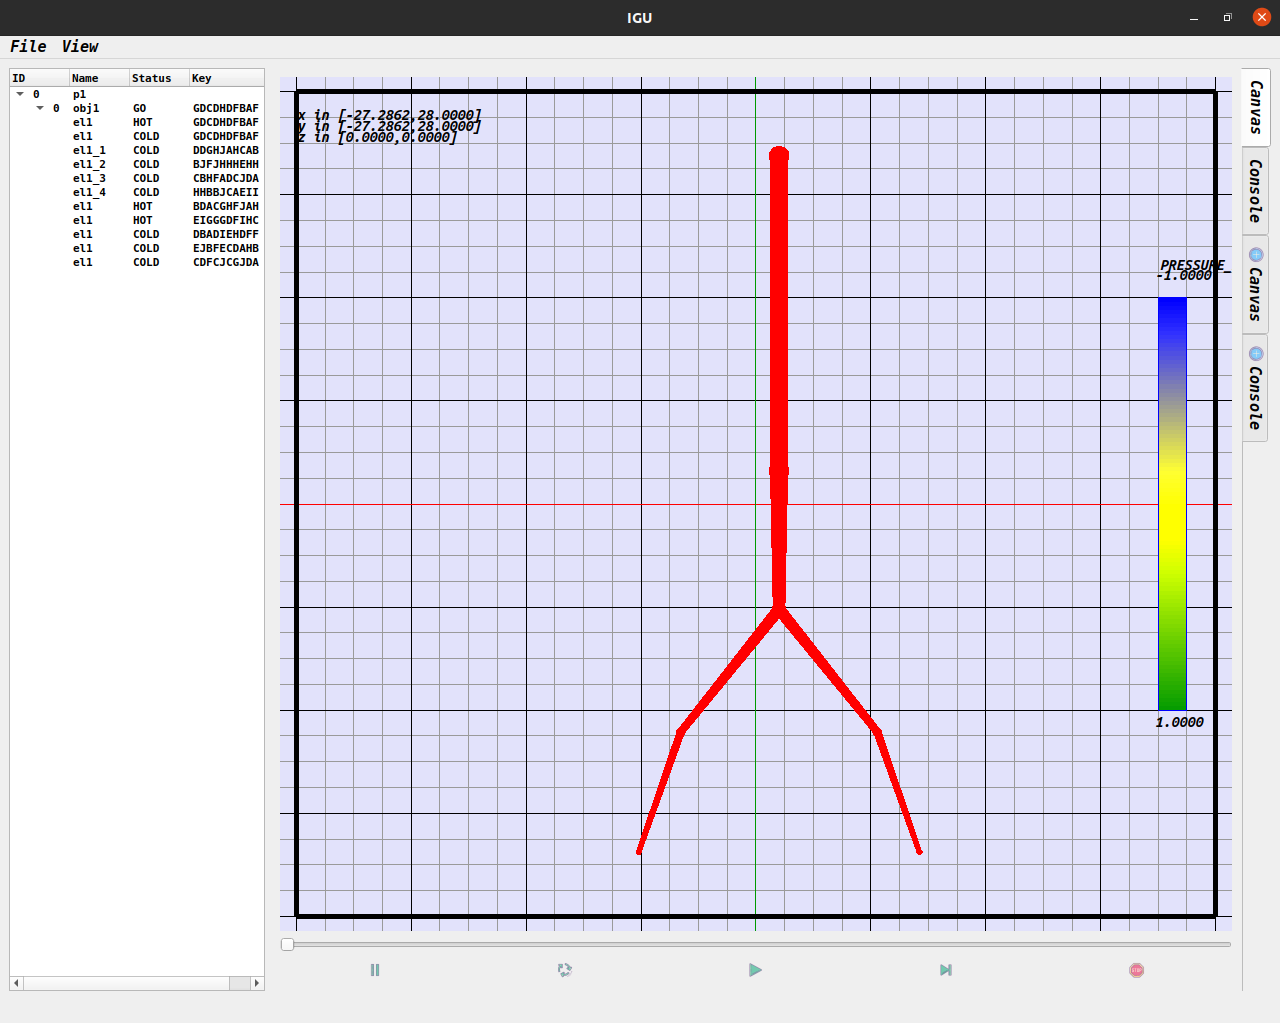
\includegraphics[scale=0.25]{Figures/IGU.png}
	\caption{Interface gráfica da ferramenta desenvolvida.}
	\label{fig1:gui}
\end{figure}

Através da modelagem de classes no paradigma do C++ \cite{AlanParker}, foi possível realizar diversas generalizações que ampliam a adaptabilidade dos objetos que podem ser inseridos neste modelo de classes. Na seção seguinte apresentamos um esquema de classes virtuais, ou abstratas, que foram criadas para facilitar o manuseio dos objetos dentro do ambiente computacional e prover funções básicas. 

Uma classe virtual não possui construtor próprio, porque classes virtuais são incompletas. Estas classes possuem métodos virtuais, que por sua vez precisam ser definidos pela classe herdeira. Portanto uma classe virtual funciona como um conjunto de regras que classes herdeiras devem seguir, todas as classes que implementem esta classe virtual devem ter sua própria definição dos métodos virtuais, podendo ter funcionamentos distintos, entretanto recebendo os mesmo parâmetros.  Utilizando este conceito a estrutura de dados, classes virtuais generalizaram os objetos e garantem o seu funcionamento, separando as estruturas de acordo com seu propósito em classes.

%--------------------------------------------------------------------------------%
\section{Estrutura de Dados}\label{sec:estrutura}

Nesta seção apresentam-se detalhes da estrutura de dados adotada no funcionamento da ferramenta computacional. Como mencionado na Seção~\ref{sec:algoritmo} é utilizada uma estrutura de ponteiros que é capaz de armazenar todas as informações do modelo geométrico da árvore arterial. A ferramenta computacional foi desenvolvida para ser capaz de armazenar, carregar e iterar o modelo matemático e gerar novas estruturas para visualização.

As seções à seguir descrevem a estrutura de dados genérica, sendo o principal objeto de estudo o fluxo pulsátil enquanto atravessa uma estrutura de árvore arterial e a visualização de seus resultados. Em versões anteriores, a ferramenta computacional  definia seus modelo matemático, geométrico e de visualização em apenas uma estrutura abstrata, o que gerou classes grandes com difícil manutenção e pouca versatilidade. Isto porque o mesmo objeto ficava responsável por diversas funções, era capaz de se instanciar, iterar e desenhar na tela através de diretivas OpenGL. Portanto, nesta versão da ferramenta computacional as classes seguem o conceito de propósito único, cujo objetivo é garantir que as classe tenham uma função apenas para que sua implementação seja menor e mais facilmente interpretada.

Com a experiência adquirida previamente três principais fluxos foram identificadas:  A iteração dos objetos, uma vez carregados estes objetos são duplicados e então atualizados por algoritmos, resultando em um objeto no estado original e um objeto atualizado pelo algoritmo; O armazenamento dos objetos, os elementos criados no método de iteração podem ser armazenados em um cache e então recuperados;  E a exibição dos objetos, uma vez carregados os objetos podem ser exibidos na tela e visualizados. Entendendo o método iterativo como uma animação em que todos os quadros precisavam ser armazenados, o objeto inteligente \textit{WiseObject} foi criado representando toda a animação e o elemento inteligente \textit{WiseElement} como cada quadro da animação. Cada quadro antes de ser exibido precisa ser processado em diretivas OpenGL, o responsável sobre esse processo é o elemento gráfico \textit{GraphicObject}. Igualmente quando se tratam de animações e reproduções de vídeo, somente quadros necessários estarão em memória. 

Finalmente, estas estruturas são utilizadas pela ferramenta computacional possibilitando que modelos geométricos sejam carregados, iterados e então exibidos, sem que haja perda dos quadros ou de algum dado. Os elementos principais da estrutura de dados serão descridos nas seções que se seguem.

%--------------------------------------------------------------------------------%
\subsection{ELEMENTO INTELIGENTE}\label{sec:elemento_inteligente}

Elementos inteligentes são objetos que implementam a classe \textit{WiseElement}, o principal objetivo de um elemento inteligente é manter os dados mais recentes de um modelo geométrico e os dados necessários para o método de iteração. No caso do estudo do fluxo pulsátil consideramos que uma iteração seja a execução completa do algoritmo apresentado na Seção~ \ref{sec:algoritmo} em toda a árvore. Portanto cada elemento inteligente possuirá todas as informações do modelo geométrico de uma árvore arterial, seus segmentos e suas propriedades.

Através das malhas estruturadas e desestruturadas presentes na biblioteca \textit{VTK}(\textit{Visualization ToolKit}) é possível descrever diversas estruturas de dados através de elementos padronizados, como pontos, linhas e células. Utilizando os elementos básicas contidas nestas malhas, variáveis e ferramentas da linguagem a estrutura básica da arquitetura foi criada, presente na Figura~\ref{fig2:wiselement}.

\begin{figure}[!htbp]
	\centering
	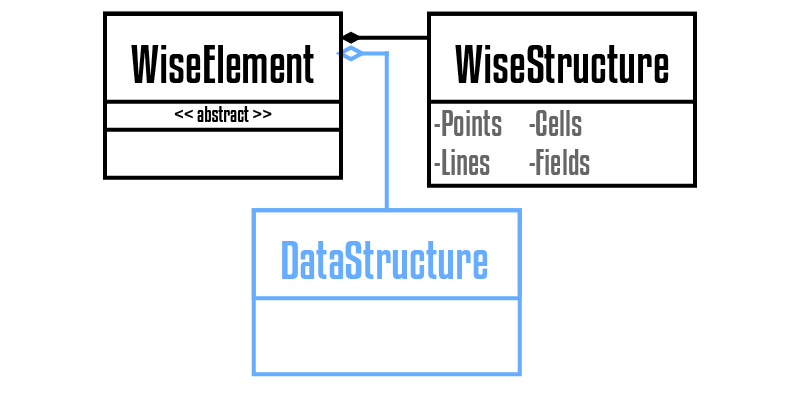
\includegraphics[scale=1]{Figures/WiseElement.png}
	\caption{Representação de classes de um elemento inteligente. WiseElement a classe abstrata base e seus componentes: WiseStructure representa a estrutura contida em um arquivo VTK e DataStructure representa a estrutura de ponteiros e variáveis utilizadas na iteração. Tingido de azul as estruturas que nem sempre estão presentes.}
	\label{fig2:wiselement}
\end{figure}

A Figura~\ref{fig2:wiselement} mostra que um elemento inteligente é composto por duas outras estruturas: A primeira \textit{WiseStructure}, utiliza pontos, linhas, células e campos para determinar estruturas geométricas; A segunda \textit{DataSructure}, representa os dados abstratos específicos de cada elemento. Estas estruturas são equivalentes entre si, isto é feito para que a estrutura siga um formato padrão de pontos, linhas, células e campos seja mantida enquanto dados abstratos equivalentes podem ser utilizados. Os dados mantidos na estrutura padrão \textit{WiseStructure} são utilizados principalmente na leitura e escrita de objetos, portanto são mantidos como cadeias de caracteres. Enquanto os dados abstratos contém a mesma informação contida em variáveis da linguagem, como números inteiros, vetores, ponteiros e outros.

\begin{figure}[!htbp]
	\centering
	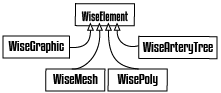
\includegraphics[scale=1]{Figures/WiseElements.png}
	\caption{Tipos de elementos inteligentes. \textit{WiseGraphic}, um gráfico bidimensional. \textit{WiseMesh}, uma malha bidimensional. \textit{WisePoly}, uma malha tridimensional. \textit{WiseArteryTree}, uma árvore arterial}
	\label{fig2:wiselements}
\end{figure}

 Como demonstrado na Figura~\ref{fig2:wiselements} um elemento inteligente é aquele que implementa a classe abstrata \textit{WiseElement}, os dados abstratos \textit{DataStructure} de cada classe podem ser salvos na estrutura padrão \textit{WiseStructure} e utilizados quando necessário. 
 
 O modelo geométrico de uma árvore arterial foi traduzido para o elemento inteligente \textit{WiseArteryTree}, a estrutura inteligente deste elemento conta com pontos e linhas que definem os parâmetros do modelo geométrico na estrutura \textit{WiseStructure}, a estrutura abstrata \textit{DataStructure} conta com ponteiros para cada segmento e grandezas físicas armazenadas em pontos flutuantes de precisão dupla.
 
O elemento inteligente \textit{WiseGraphic} foi criado para armazenar dados ao longo de uma dimensão, como a pressão ao longo da árvore arterial. Os elementos \textit{WiseMesh} e \textit{WisePoly} foram criados para armazenar dados ao longo de duas dimensões e ao longo de três dimensões, estes dois elementos foram utilizados como exemplo de objetos que podem ser generalizados na ferramenta e visualizados, mudando pouco as estruturas já existentes. O elemento \textit{WiseGraphic} é equivalente à um vetor de valores $(x,v)$, o elemento \textit{WiseMesh} à uma matriz de valores $(x,y,v)$ e o elemento \textit{WisePoly} uma matriz tridimensional de valores $(x,y,z,v)$, onde $v$ é o valor associado e $(x,y,z)$ a posição. Podemos armazenar em um \textit{WiseMesh} o valor $v$ da pressão ao longo de uma árvore arterial na direção $x$ variando a frequência no eixo $y$, por exemplo.
 
 Os elementos inteligentes servem como estruturas de armazenamento padrão que compõem outros objetos. O ciclo de manipulação desses elementos se divide em três partes: A criação, aonde os objetos podem ser criados à partir de exemplos pré-definidos ou através de um arquivo de entrada \textit{VTK} ou \textit{XML (eXtensible Markup Language)}; A iteração, processo em que o elemento inteligente com todas as estruturas definidas e consistentes é utilizado por um algoritmo; A exibição,  este último ciclo utiliza a estrutura atualizada e gera um objeto para visualização.
 
Todo elemento inteligente completo possui uma redundância de dados, podendo ser representado por qualquer uma das duas estruturas que o compõe. A estrutura \textit{WiseStructure} utiliza componentes simples para descrever as estruturas e seus parâmetros, essa estrutura é a que mais se assemelha à encontrada na arquitetura \textit{VTK}. Por utilizar uma quantidade limitada de diretivas o arquivo proveniente dessa estrutura pode ser rapidamente lido, interpretado e até mesmo exportado.

\begin{figure}[!htbp]
	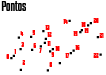
\includegraphics[width=0.33\textwidth]{Figures/WiseElementPoints.png}
	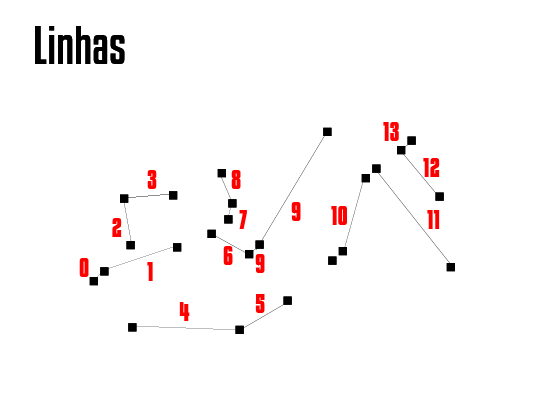
\includegraphics[width=0.32\textwidth]{Figures/WiseElementLines.png}
	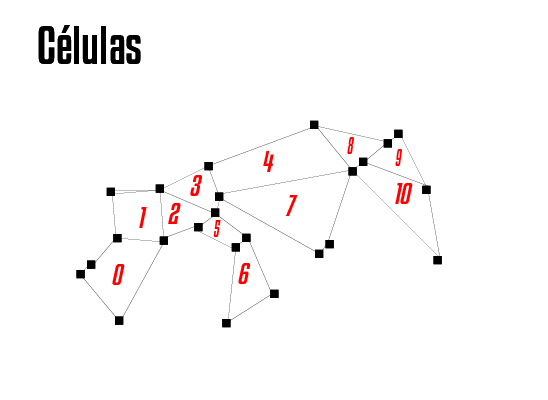
\includegraphics[width=0.33\textwidth]{Figures/WiseElementCells.png}
	\caption{Pontos utilizados na especificação do modelo geométrico. Linhas utilizadas na especificação do modelo geométrico, através dos pontos previamente definidos. Células utilizadas na especificação do modelo geométrico, através dos pontos previamente definidos.}
	\label{fig2:wiselementstructs}
\end{figure}

Os componentes de uma estrutura inteligente são pontos, células, linhas e campos. Pontos demarcam uma posição no espaço, células e linhas representam conjuntos de pontos e os campos são dados gerais da estrutura. Um modelo de pontos e linhas é capaz de representar o mesmo modelo geométrico de uma árvore arterial, basta considerar cada ponto uma bifurcação de vasos e cada segmento de vaso uma linha. Através destes componentes simples é possível armazenar e acessar dados sobre cada ponto e linha, armazenando dados de cada segmento pertencente à uma árvore arterial através da estrutura \textit{WiseStructure}. Para dados gerais do modelo, como a frequência $f$, os campos da estrutura inteligente são utilizados.

A classe \textit{WiseElement} foi desenvolvida para construir a estrutura abstrata (\textit{DataStructure}) à partir das informações contidas na estrutura inteligente (\textit{WiseStructure}), desta forma é importante que a estrutura inteligente possa rapidamente ser armazenado e recuperado. O elemento inteligente é o elemento básico do método de iteração, antes de ser iterado este elemento é duplicado, gerando estruturas inteligente e abstrata idênticas. Imediatamente a estrutura abstrata \textit{DataStructure} é descartada e os dados contidos na estrutura padrão \textit{WiseStructure} são armazenados. Portanto, a estrutura abstrata não estará sempre presente. Seguindo este ciclo de vida, todos os elementos inteligentes obedecem à máquina de status contida na Figura~\ref{fig3:wiselementstatus}.

\begin{figure}[!htbp]
	\centering
	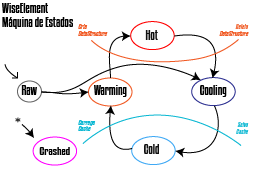
\includegraphics[scale=1.5]{Figures/WiseElementStatus.png}
	\caption{Máquina de Status que controla o funcionamento de um elemento inteligente.}
	\label{fig3:wiselementstatus}
\end{figure}

A máquina de status dos elementos inteligentes gerencia o ciclo de vida de todos os elementos inteligentes, elementos inicialmente recebem o estado \textit{Raw}, ou cru, que representa um elemento ainda sem estruturas carregadas ou sem consistência garantida. Uma vez que a estrutura inteligente é inserida e verificada o elemento muda para o status \textit{Warming} ou \textit{Cooling}, respectivamente esquentando ou esfriando, suas estruturas são representadas na Figura~\ref{fig4:wiselementwarming}.

\begin{figure}[!htbp]
	\centering
	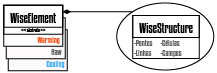
\includegraphics[scale=1]{Figures/WiseElementWarming.png}
	\caption{Elemento inteligente enquanto no estado \textit{Warming}.}
	\label{fig4:wiselementwarming}
\end{figure}

A figura~\ref{fig4:wiselementwarming} mostra as estruturas presentes em elementos no estado \textit{Warming} que é a mesma dos estados \textit{Raw} e \textit{Cooling}. Cada estado possui uma finalidade diferente e representa em que estado estão as informações do elemento inteligente. Elementos no estado \textit{Warming} estão aguardando a construção de sua estrutura abstrata, enquanto elementos  no estado \textit{Cooling} aguardam que seus dados sejam salvos em cache. Finalmente, elementos no estado \textit{Raw} indicam que não é esperada a consistência dos dados.

Inicialmente os elementos inteligentes são criados no estado \textit{Raw}, enquanto os dados do elemento são carregados ele permanecerá neste estado. Ao final do carregamento o objeto trocará de estado para \textit{Warming} ou \textit{Cooling}, que indicam o próximo passo do elemento. Estar no estado \textit{Warming} indica que o objeto irá criar a sua estrutura de dados abstrata, enquanto o estado \textit{Cooling} indica que a estrutura inteligente aguarda ser armazenada. Quando os dados abstratos são criados corretamente para a estrutura o estado é definido como \textit{Hot}, neste estado todas as informações do objeto estão em memória, sendo este o estado mais pesado do elemento inteligente. Em contraponto, o estado \textit{Cold} indica que a estrutura inteligente foi corretamente armazenada em disco, elementos inteligentes neste estado estão em seu estado mais leve, pois possuem em memória apenas o caminho para a estrutura inteligente armazenada.

Como demonstrado na figura~\ref{fig3:wiselementstatus}, o estado frio (\textit{Cold}) está associado com o uso de um cache para estruturas inteligentes. A estrutura do arquivo é equivalente à uma malha estruturada VTK, mas são efetivamente salvos em um arquivo \textit{XML}. Caso sejam novamente carregados por uma mudança de estado ou deletados o arquivo armazenado é deletado. Quando um elemento inteligente está neste estado ele contém apenas o endereço para o arquivo em que foi armazenado.

\begin{figure}[!htbp]
	\centering
	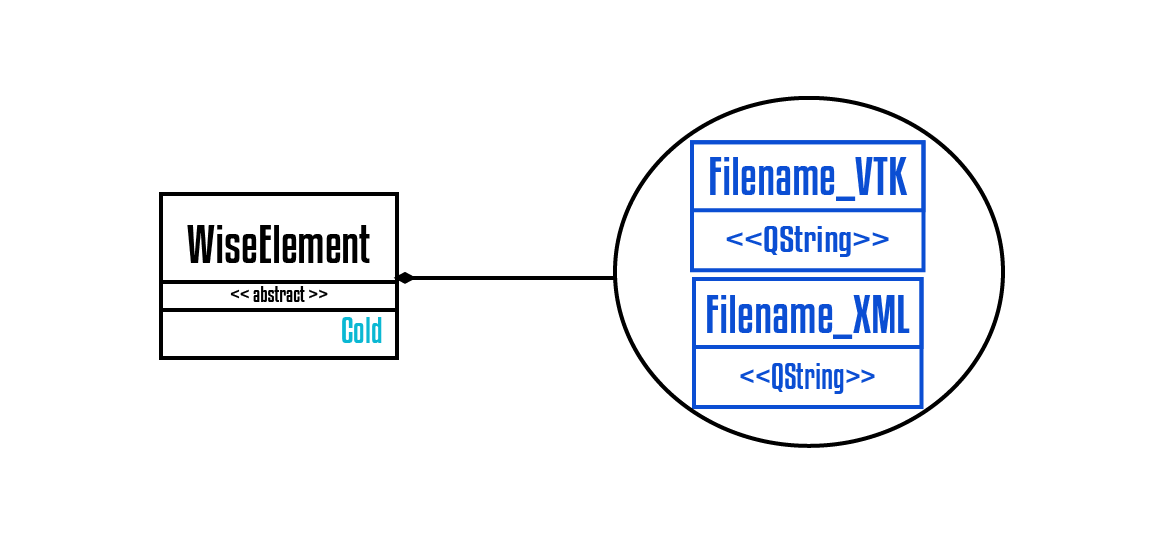
\includegraphics[scale=1]{Figures/WiseElementCold.png}
	\caption{Elemento inteligente enquanto no estado \textit{Cold}.}
	\label{fig5:wiselementcold}
\end{figure}

O estado \textit{Crashed} serve para identificar objetos que não tem mais o funcionamento esperado. Durante a troca de estados do elemento é verificado se os elementos esperados estão presentes, caso não estejam o objeto é direcionado à este estado.

Finalmente, o estado \textit{Hot} representa os elementos que possuem todas as estruturas presentes. Isto significa que a estrutura inteligente \textit{WiseStructure} e a estrutura abstrata equivalente \textit{DataStructure} estão presente e são consistentes.

\begin{figure}[!htbp]
	\centering
	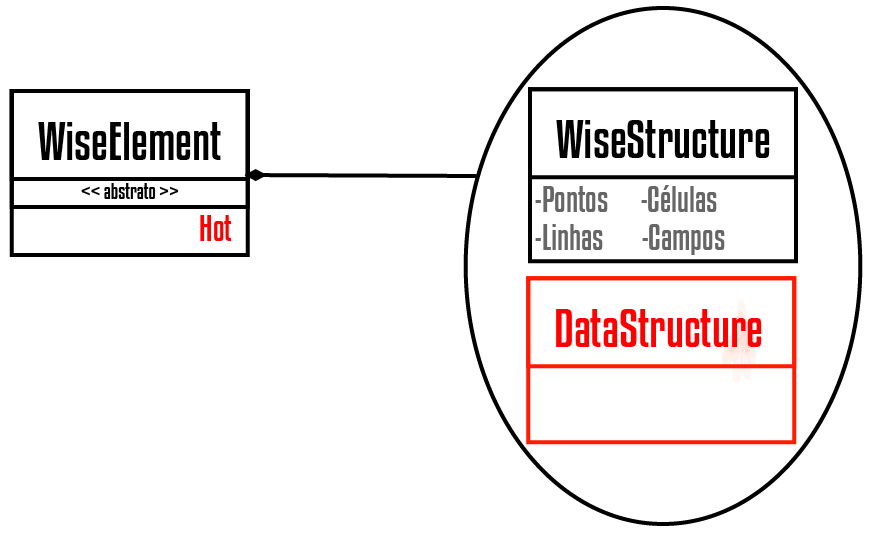
\includegraphics[scale=1]{Figures/WiseElementHot.png}
	\caption{Elemento inteligente enquanto no estado \textit{Hot}.}
	\label{fig6:wiseelementhot}
\end{figure}

Para que um elemento possa ser iterado ele precisa estar no estado \textit{Hot}, porque durante a iteração de um elemento inteligente seus dados abstratos são utilizados. A cada passo da iteração a estrutura \textit{DataStructure} é atualizada, exigindo uma atualização da estrutura \textit{WiseStructure}.

Seguindo o conceito de classes com propósito único, os elementos inteligentes são responsáveis apenas por gerir os dados contidos na estrutura inteligente e abstrata. Portanto as funções de criar, iterar e visualizar estas estruturas foram divididas em classes.

%--------------------------------------------------------------------------------%
\subsection{FÁBRICA}\label{sec:fabrica} 
 
Como mencionado anteriormente três principais barreiras foram identificadas armazenamento, iteração e visualização. Foi idealizada uma arquitetura de classes que permite a execução de cada passo através do paradigma de Fábricas Dinâmicas~ \cite{factorypattern}. Uma arquitetura com fábricas permite a criação de instâncias com definições concretas, armazenadas como metadados. Isso facilita a adição de novos objetos que podem ser interpretados sem modificar o código da fábrica em si. Sendo a fábrica também uma classe virtual, três principais tipos de fábricas foram idealizadas, a primeira responsável por criar elementos inteligentes, a  segunda responsável por iterar o elemento e a terceira que cria um elemento gráfico a partir de um elemento inteligente.

\begin{figure}[!htbp]
	\centering
	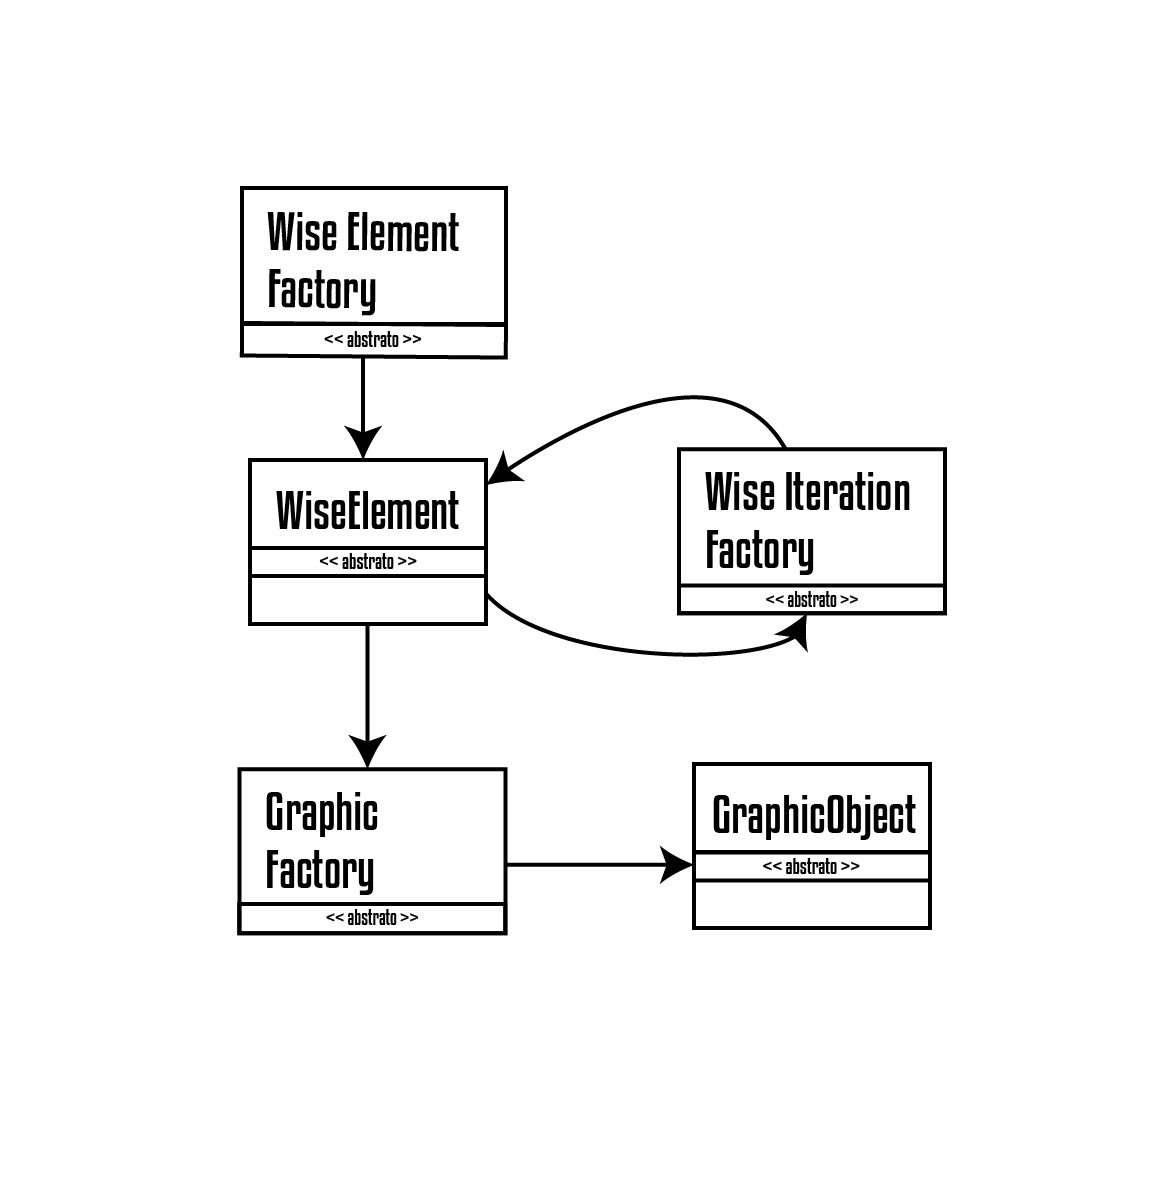
\includegraphics[scale=1]{Figures/WiseElementWorkflow.png}
	\caption{Arquitetura de classes fábrica e fluxo de trabalho do elemento inteligente WiseElement. A fábrica WiseElementFactory é responsável por criar o elementos inteligentes, a fábrica WiseIterationFactory é reponsável pela iteração do elemento inteligente e a fábrica GraphicFactory é responsável por criar as estrturas de visualização. }
	\label{fig2:wiselementsworkflow}
\end{figure}
 
Primeiramente, a fábrica de elementos inteligentes \textit{WiseElementFactory} é utilizada para a criação de elementos inteligentes, essa fábrica é utilizada para criar um elemento inteligente à partir de parâmetros. Esse tipo de fábrica é também uma classe virtual, seus métodos definem que fábricas de elementos inteligentes possuem três maneiras de executar: Um dos métodos permite a criação de elementos à partir de uma lista de exemplos; Outro método permite que um arquivo \textit{VTK} ; Com um arquivo \textit{XML}. 

Os métodos de criação de elementos são selecionados através do nome da fábrica e de um dos três métodos de criação. A ferramenta computacional possui uma lista com todas a fábricas disponíveis e as utiliza quando necessário. Devido à forma como os dados são carregados para cada elemento, é necessário que haja uma fábrica para cada tipo de elemento inteligente.

A fábrica \textit{WiseIterationFactory} só pode operar com um tipo específico de elemento inteligente, entretanto é possível que haja mais de uma fábrica de iteração disponível por tipo de elemento inteligente. Desta forma uma árvore arterial pode ser iterada por diferente algoritmos de iteração e o mesmo ocorre com os outros tipos de elementos. Estas fábricas são responsáveis por executar algum algoritmo que utilize o tipo de dados do elemento inteligente. No caso de uma árvore arterial é possível utilizar uma fábrica que irá executar o modelo matemático descrito na seção~\ref{sec:algoritmo} utilizando os ponteiros para segmentos disponíveis em uma \textit{WiseArteryTree}.

Por último, a fábrica \textit{GraphicFactory} irá criar o objeto gráfico correspondente ao elemento inteligente. Assim como um elemento inteligente um objeto gráfico pode ser salvo em cache.  Um elemento inteligente é composto por todas as linhas, pontos, células e seus valores associados, enquanto um objeto gráfico contém as representações gráficas destes elementos e para cada um armazena um valor. Os elementos estruturais de uma árvore arterial, que são seus pontos e linhas, são traduzidos em círculos e cilindros como visto na Figura~\ref{fig1:gui} . Sobre estes elementos gráficos apenas um valor pode ser exibido por vez ao longo da escala de cores, como o fluxo $Q$ ou a pressão $P$. Dessa forma os elementos gráficos só exigem que um parâmetro por vez sejam armazenados.


%--------------------------------------------------------------------------------%
\subsection{OBJETO INTELIGENTE}\label{sec:objeto_inteligente}

A classe que combina todas as estruturas utilizadas no método de iteração da ferramenta computacional foi nomeada de objeto inteligente \textit{WiseObject}, este objeto preserva todos os passos de de iteração e poupa a quantidade de recursos mantida em memória. A classe é composta por um coleção de elementos inteligentes e objetos gráficos equivalentes entre si. A presença de uma fábrica gráfica é opcional, possibilitando que objetos sejam iterados sem que alguma estrutura seja disponibilizada para visualização. Utilizando a mesma separação de classes com propósito único, fábricas dinâmicas garantem que um objeto inteligente seja criado corretamente. As fábricas presente na Seção~\ref{sec:fabricas} foram incluídas como propriedades de um objeto inteligente, desta forma estes objetos serão compostos por três fábricas.

O ciclo de vida de um objeto inteligente consiste na sua criação, a iteração de um modelo matemático e, opcionalmente, a exibição de um modelo gráfico. Objetos inteligentes são criados com seu primeiro elemento inteligente. Ao criar um objeto inteligente, sua fábrica adiciona em sua estrutura a fábrica de elementos inteligentes, desta forma objetos inteligentes são capazes de replicar seus elementos inteligentes. No momento da da criação, o primeiro elemento é duplicado e uma instância segue para o \textit{Forno}, enquanto a outro segue para o \textit{Freezer}.

O elemento inteligente guardado no \textit{Forno} será o objeto utilizado pelo algoritmo a cada iteração, sendo o mais atual. A cada ciclo o elemento contido no \textit{Forno} é duplicado e uma nova instância é adicionada ao \textit{Freezer}, estes elementos serão armazenados.

\begin{figure}[!htbp]
	\centering
	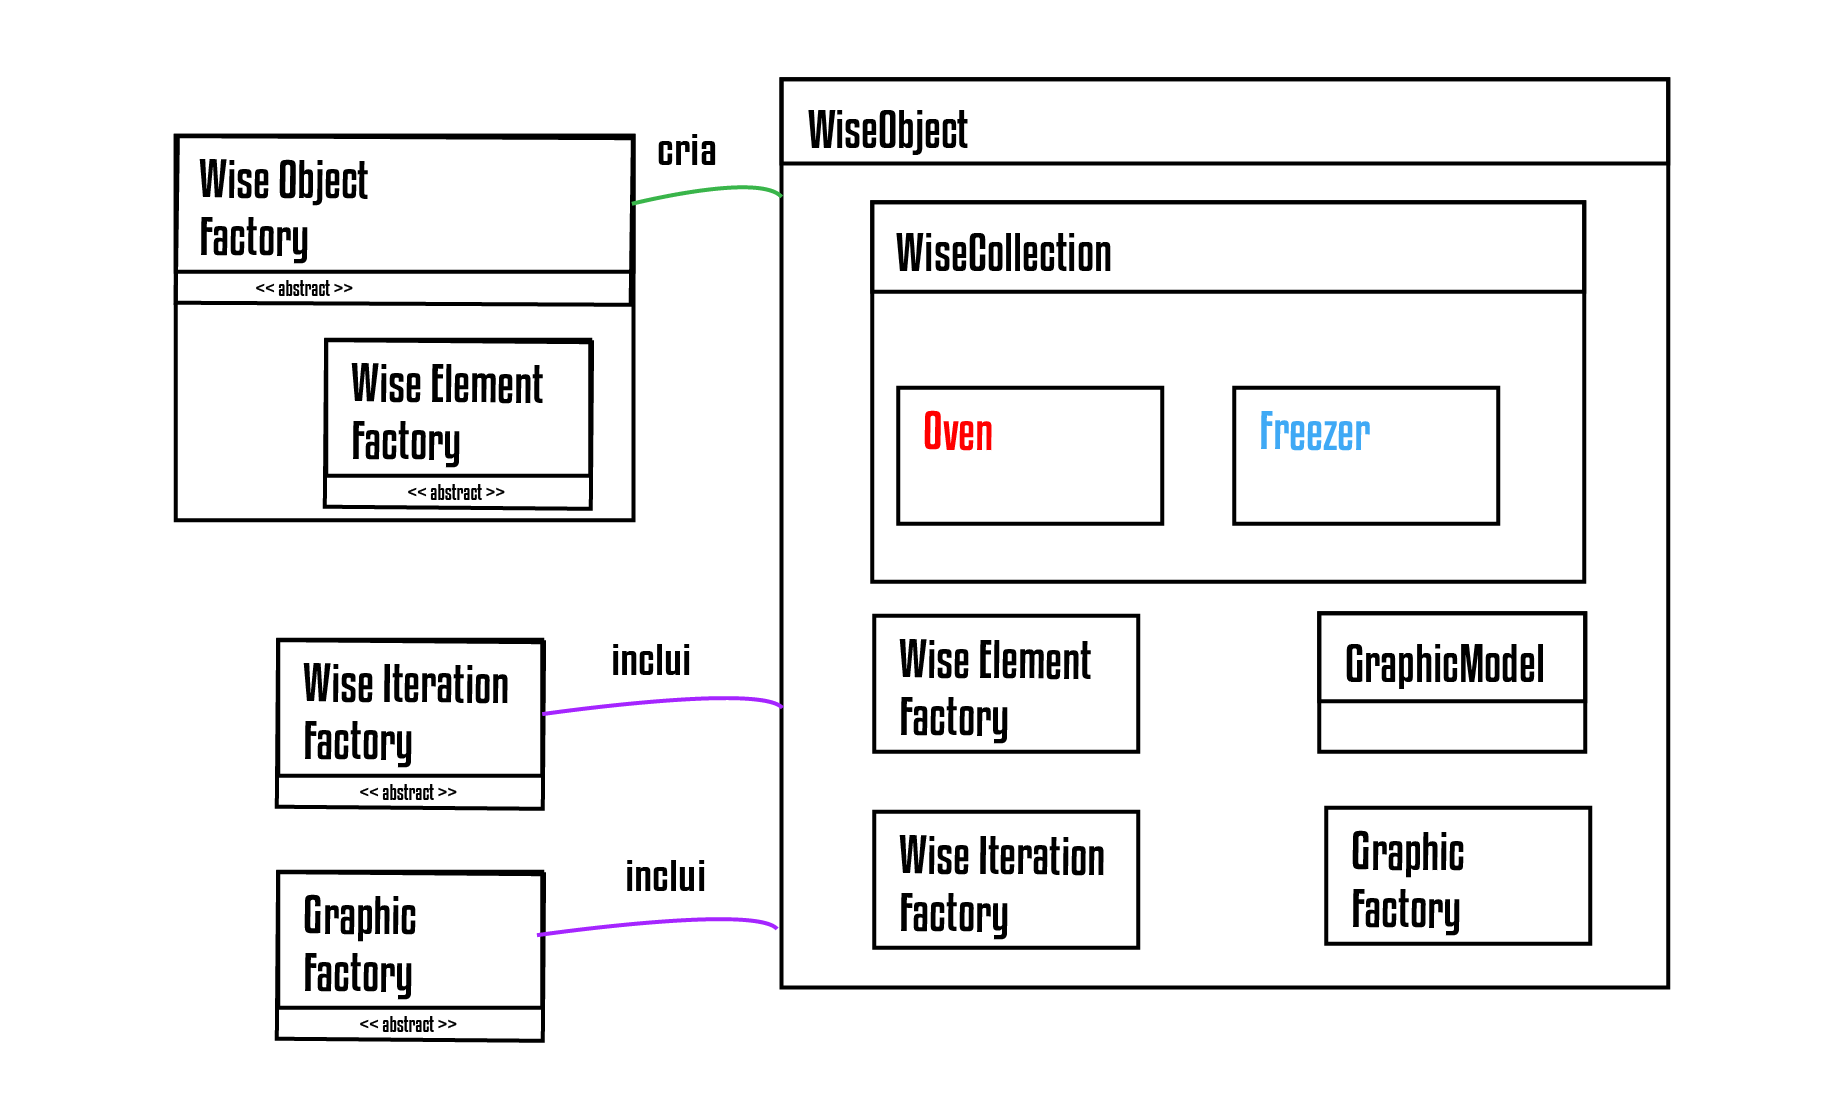
\includegraphics[scale=1]{Figures/WiseObject.png}
	\caption{Objeto inteligente \textit{WiseObject} e todos seu componentes:\textit{WiseObjectFactory}, fábrica responsável pela criação de objetos inteligentes de um predeterminado tipo; \textit{WiseIterationFactory}, fábrica de iteração; \textit{WiseGraphicFactory}, fábrica gráfica; \textit{WiseCollection}, coleção de elementos inteligentes; \textit{GraphicModel}, coleção de objetos gráficos.}
	\label{fig7:wiseobject}
\end{figure}

Através do modelo de classes de um objeto inteligente presente na Figura~\ref{fig7:wiseobject} é possível identificar todos os componentes presentes em um objeto inteligente. O objeto inteligente troca seus elementos de estado automaticamente, a coleção de elementos inteligentes \textit{WiseCollection} irá manter apenas um elemento em memória, o elemento contido no \textit{Forno} que deve permanecer no estado \textit{Hot}. Ao mesmo tempo a coleção irá manter um históricos de elementos armazenados no \textit{Freezer} que devem permanecer no estado \textit{Cold}. É possível que o objeto inteligente volte à um estado anterior, substituindo o elemento presente no \textit{Forno} com algum estado anterior armazenado no \textit{Freezer}, dessa forma o elemento inteligente utilizado no método iterativo será o objeto recuperado. Ao realizar essa operação, a coleção de elementos inteligentes irá recuperar a estrutura inteligente do elemento, alterando seu estado para \textit{Warming}. Em seguida irá recriar os seus dados abstratos utilizando uma das fábricas disponíveis, alterando seu estado para \textit{Hot}.

Objetos inteligentes também tem seu funcionamento descrito por uma máquina de estados. Para definir corretamente os resultados do método de iteração utilizando a estrutura do objeto inteligente, uma sequência de passos foi criada: os dados são instanciados em objetos inteligentes, os dados são ajustados para cada experimento, uma sequência de iterações é executada e finalmente os objetos são descartados.

\begin{figure}[!htbp]
	\centering
	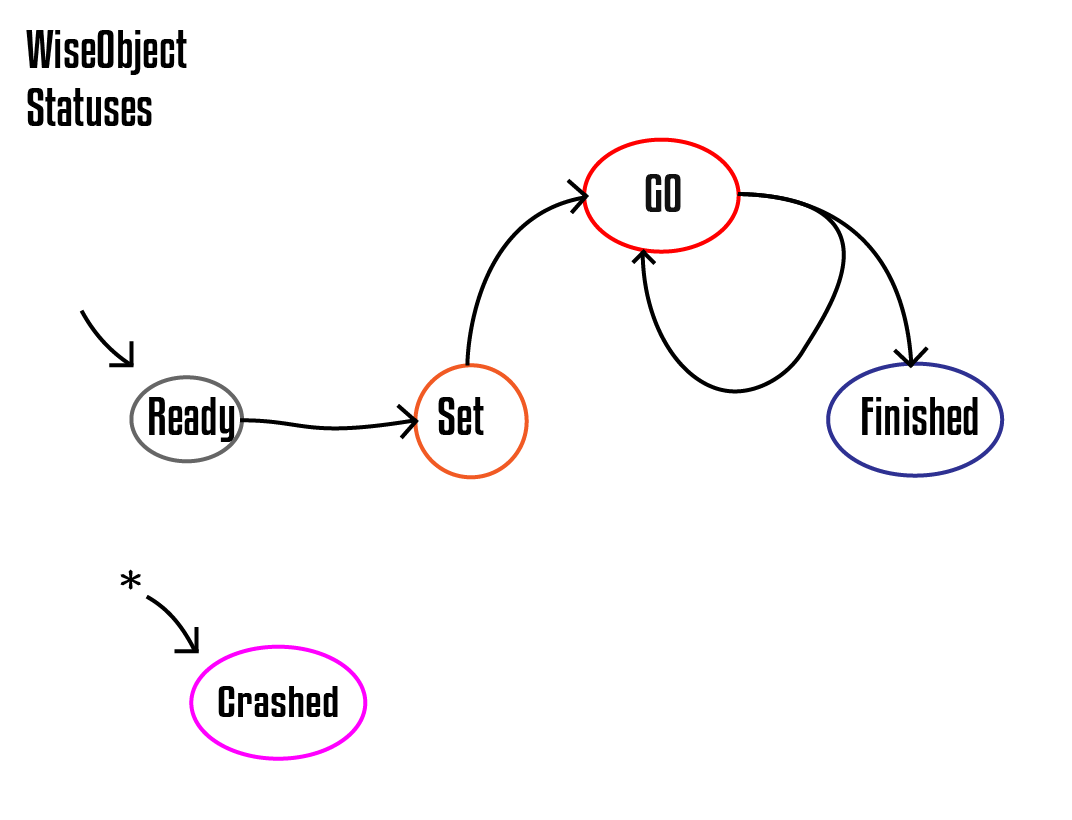
\includegraphics[scale=1]{Figures/WiseObjectStatus.png}
	\caption{Modelo gráfico \textit{GraphicModel}, contém uma coleção de objetos gráficos.}
	\label{fig7:wiseobjectstatuses}
\end{figure}

As trocas de estado dos objetos inteligentes são causadas por operações do usuário para preparar o objeto para iteração e para executar o método de iteração. Desta forma o usuário pode definir quais fábricas serão inseridas no objeto, parâmetros do modelo geométrico e do experimento e quais trocas de estados devem ser executadas.

Como objetos inteligentes são criados à partir de um elemento inteligente, eles possuem os mesmos métodos de criação. As fábricas de objetos inteligentes \textit{WiseObjectFactory} são compostas por fábricas de elementos inteligentes \textit{WiseElementFactory}. É possível criar objetos inteligentes de duas formas, utilizando um elemento inteligente já existente ou utilizar os métodos de criação de elementos disponíveis na fábrica de elementos inteligentes.

Em seguida é necessário definir qual será a lógica de iteração do objeto, adicionando uma fábrica de iteração \textit{WiseIterationFactory} compatível. Para o caso de escoamento pulsátil através de uma árvore arterial é necessário se adicionar a fábrica de iteração correspondente ao algoritmo da Seção~\ref{sec:algoritmo} e em seguida definir os parâmetros desejados, como a frequência $f$, a viscosidade $\mu$ e o ângulo de fase $\phi$. Com as alterações concluídas o objeto passa a poder ser iterado, opcionalmente a fábrica gráfica \textit{GraphicFactory} pode ser inserida. Caso seja incluída, o objeto inteligente passará a gerar objetos gráficos \textit{GraphicObject} a cada iteração.

Inicialmente, um objeto é criado no estado \textit{Ready} com somente seu elemento inicial e uma fábrica do tipo \textit{WiseElementFactory}. Neste estado é esperada a inclusão das fábricas de iteração e gráficas. Uma vez que elas estejam corretamente acopladas ao objeto inteligente, é possível fazer a troca do estado \textit{Ready} para o estado \textit{Set}. Com a mudança de estado, é adicionado à estrutura inteligente \textit{WiseStructure} todos os parâmetros disponibilizados pela fábrica de iteração e gráfica. Um objeto no estado \textit{Set} indica que o objeto foi corretamente criado, uma fábrica de iteração foi adicionada, possivelmente uma fábrica gráfica e agora aguarda alterações nestes parâmetros ou execução do método iterativo.

Com os parâmetros definidos e as fábricas devidamente acopladas os objeto está pronto para a iteração. O método iterativo de um objeto inteligente é representado na transição para o estado \textit{Go}. Uma iteração de uma \textit{WiseArteryTree} representa o cálculo dos valores de pressão e fluxo em toda a árvore arterial. Caso algum erro ocorra durante o processamento de dados o objeto se desloca para o estado \textit{Crashed}, assim como elementos inteligentes. É possível também finalizar a execução de um objeto inteligente o enviando para o estado \textit{Finished}, neste estado o objeto não poderá ser iterado novamente. O objeto inteligente também pode ser reiniciado à partir de qualquer estado, o que significa que todas as alterações feitas na estrutura do objeto inteligente serão apagadas. Para que parâmetros da iteração possam ser alterados sem que se perda elementos inteligentes até então definidos, é possível que um objeto no estado \textit{Go} seja resetado e retorne para o estado \textit{Set}.

%--------------------------------------------------------------------------------%
\subsection{OBJETO GRÁFICO}\label{sec:objeto_grafico}


Quando o objeto inteligente \textit{WiseObjet} estiver corretamente carregado e uma fábrica gráfica \textit{GraphicFactory} for adicionada à sua estrutura o primeiro objeto gráfico \textit{GraphicObject} de sua coleção será criado. Assim como o elemento inteligente representa uma iteração, um objeto gráfico representa um ciclo iterativo. Enquanto a estrutura responsável por elementos inteligentes, \textit{WiseCollection}, é responsável por manter os últimos dados de iteração aquecidos, a estrutura \textit{GraphicModel} mantém o objeto que está sendo exibido por alguma tela e elementos próximos. As coleções tem como objetivo mantes seus elementos no estado necessário e realizar trocas de estados quando necessário. No caso dos elementos inteligentes, somente o último objeto é necessário e isso não muda, no contexto dos objetos gráficos apenas o objeto exibido em um elemento da interface de usuário e seus vizinhos serão mantidos em memória.

\begin{figure}[!htbp]
	\centering
	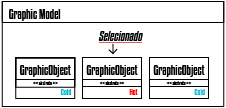
\includegraphics[scale=1]{Figures/GraphicModel.png}
	\caption{Modelo gráfico \textit{GraphicModel}, contém uma coleção de objetos gráficos.}
	\label{fig7:graphicmodel}
\end{figure}

Presente na Figura~\ref{fig7:graphicmodel} estão os componentes que permitem armazenar todos os quadros da animação final. Quando um objeto \textit{WiseObject} está corretamente configurado com uma instância de fábrica gráfica \textit{GraphicFactory}, seu método iterativo é atrelado à criação de objetos gráficos. Isso permite que o objeto iterado crie um elemento inteligente \textit{WiseElement} e um objeto gráfico \textit{GraphicObject} à cada iteração.

\begin{figure}[!htbp]
	\centering
	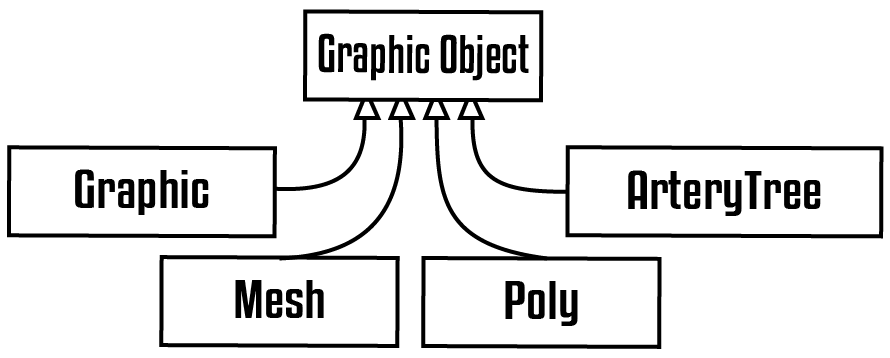
\includegraphics[scale=1]{Figures/GraphicObjects}
	\caption{Tipos de objetos gráficos \textit{GraphicObjects}.}
	\label{fig7:graphicobjects}
\end{figure}

Cada objeto gráfico se desenha através de diretivas OpenGL, o formato do modelo geométrico é apresentado ao usuário através das formas desenhadas, enquanto algum parâmetro do elemento inteligente \textit{WiseElement} é visualizado através de uma escala de cores.

Os objetos gráficos contidos na Figura~\ref{fig7:graphicobjects} possuem métodos específicos para se desenhar utilizando um gradiente de cores e formas geométricas padrão, bidimensionais ou tridimensionais. Cada forma geométrica utilizada é representada por elementos gráficos \textit{GraphicElement}, elementos que implementam a classe virtual \textit{GraphicElement}. Cada elemento gráfico é atrelado à um valor ou à uma lista de valores, estes valores são selecionados pela fábrica gráfica e adicionados a cada iteração, retirando a informação do elemento inteligente atual. Cada objeto gráfico possui um valor máximo e mínimo que é vinculado ao gradiente cores, com isso as cores representam os valores armazenados em cada objeto gráfico.

\begin{figure}[!htbp]
	\centering
	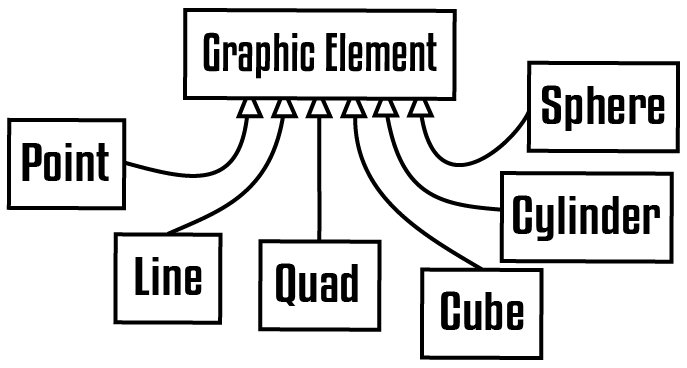
\includegraphics[scale=1]{Figures/GraphicElements}
	\caption{Tipos de elementos gráficos \textit{GraphicElements}. \textit{Point}, um ponto. \textit{Line}, uma linha. \textit{Quad}, um quadrado. \textit{Cube}, um cubo. \textit{Cylinder}, um cilindro. \textit{Sphere}, uma esfera.}
	\label{fig7:graphicelements}
\end{figure}

Os elementos gráficos podem ser utilizados por qualquer tipo de objeto gráfico. A representação geométrica de uma árvore arterial é construída utilizando cilindros e esferas, que representam segmentos de vaso e terminais, respectivamente. Por padrão, os cilindros receberão uma lista de valores da pressão $P(X) \forall X \in [0,1]$, enquanto as esferas receberão os valores da pressão $P(X)$ quando $X=0$ ou $X=1$, condicionado a escolha do nó distal($X=1$) ou o nó proximal($X=0$).  Assim como os objetos inteligentes \textit{WiseObject} têm seus tipos definidos pelo tipo de elemento inteligente que o compõe, o objeto gráfico \textit{GraphicObject} tem seu tipo definido pelo elemento inteligente que representa, com sua fábrica própria.

Apesar do objeto gráfico \textit{GraphicObject} ser uma redundância dos dados armazenados em um elemento inteligente \textit{WiseElement}, ele é menor, podendo ser carregado e armazenado mais rapidamente. O objetivo das estruturas nesta seção é permitir que diversos objetos gráficos \textit{GraphicObjects} possam ser armazenados em memória. Os objetos gráficos em sequência representam uma animação que pode ser visualizada através da interface gráfica. 


%--------------------------------------------------------------------------------%
\subsection{FÁBRICAS}\label{sec:fabricas} 



%--------------------------------------------------------------------------------%
\subsection{THREADS INTELIGENTES}\label{sec:threads}

Até o momento as estruturas foram construídas utilizando conceitos padrões da linguagem C++, herança de propriedades através do polimorfismo, ponteiros, classes virtuais e fábricas dinâmicas. Todas as estruturas definidas até o momento seguem conceitos da linguagem concorrente, ondem uma instrução é executada logo após a outra. Observamos que as estruturas possuem comportamentos padronizados e que um objeto inteligente é autônomo, isto é, ele sozinho é capaz de se armazenar, reconstruir, iterar e ocasionalmente se desenhar. Imaginando um cenário em que diversos objetos inteligente estão iterando, as tarefas foram dividas em Threads, primeiramente trabalhos de leitura e escrita, em seguida a iteração dos objetos. Desta forma computadores \textit{multi-thread} podem fazer uso de suas threads e permitir que mais de um objeto realize suas tarefas por vez.

Ao longo da pesquisa esta estrutura foi agregada as bibliotecas comuns do Qt 5.15.0 \cite{QTClasses}, em um primeiro momento para facilitar a visualização dos resultados através dos elementos gráficos de interface de usuários disponibilizados. Em seguida, permitiu o processamento de elementos de forma paralela. Com isso um modelo que suportasse o processamento distribuído utilizando classes \textit{QThreads} que possuem tarefas concorrentes foi construído.


\begin{figure}[!htbp]
	\centering
	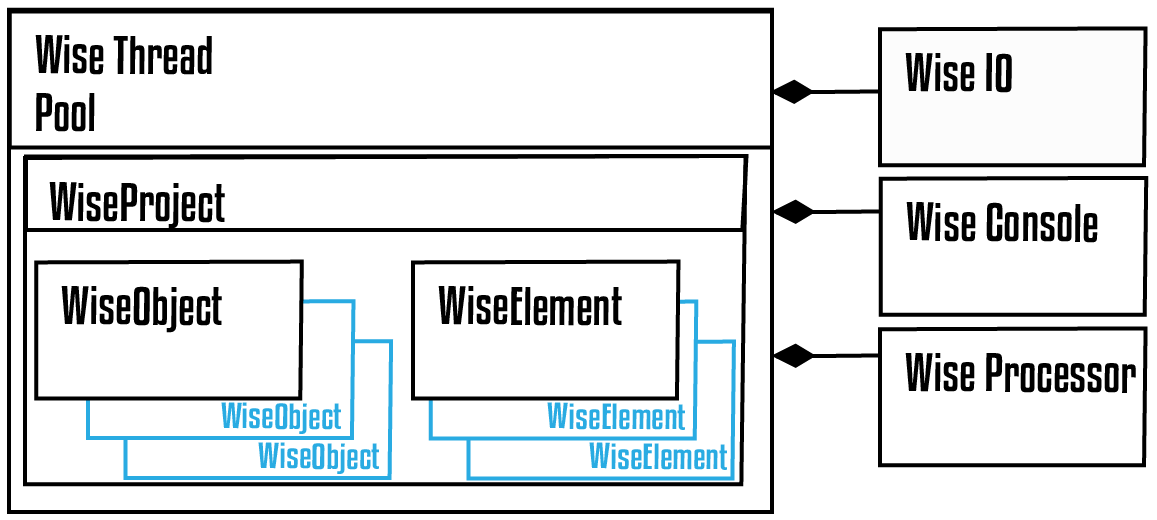
\includegraphics[scale=1]{Figures/WiseThreadPool.png}
	\caption{Modelo de Threads. \textit{WiseThreadPool}, responsável por orquestrar o funcionamento das demais threads, bem como os objetos contidos em um projeto \textit{WiseProject}. \textit{WiseIO}, thread responsável por processos de leitura e escrita. \textit{WiseConsole}, thread responsável por interpretar os comandos de texto e os traduzir em métodos. \textit{WiseProcessor}, thread responsável por realizar o método iterativo de um objeto inteligente \textit{WiseObject}}
	\label{fig7:threads}
\end{figure}

As tarefas se dividem em três principais grupos: tarefas auxiliares, tarefas de leitura/escrita e trabalhos de iteração. O principal trabalho auxiliar é interpretar os comandos recebidos pelo programa e então criar a instância de trabalho \textit{WiseJob}. Sendo os grupos de tarefas mais custosos os de tarefas de escrita/leitura e iteração, se dividiram em threads específicas, \textit{WiseIO} e \textit{WiseProcessor} respectivamente.

Os objetos distribuídos threads contidos na Figura~\ref{fig7:threads} possuem um ciclo próprio, portanto executam tarefas assíncronas e precisam de tratamento adequado. O sistema de sinais e fendas disponibilizado pelas bibliotecas comuns do Qt permitem que as threads se comuniquem assincronamente através do envio de mensagens. Estas mensagens são chamadas de trabalhos inteligentes \textit{WiseJobs}, cada uma possuindo sua atividade relacionada e objeto relacionado. Uma vez criados, os trabalhos inteligentes são alocados à sua respectiva categoria passando por um balanceamento executado pelo gerenciador de threads. Enquanto o processamento é feito, todos os dados relativos ao processamento são bloqueados para escrita de outras threads, isso previne a sobrescrita de dados quando há mais de uma thread trabalhando.

O gerenciador de threads \textit{WiseThreadPool} é composto por threads que executam os trabalhos e por projetos inteligentes \textit{WiseProject} que criam trabalhos. Ao executar um comando de texto o projeto deve ser selecionado para que os elementos e objetos certos sejam selecionados. Primeiramente, o comando será recebido pelo gerenciador e o primeiro trabalho inteligente \textit{WiseJob} será criado. Em seguida será interpretado por threads do grupo de tarefas auxiliares \textit{WiseConsole}, caso seja um trabalho de leitura, escrita ou iteração um trabalho inteligente associado será criado e enviado ao gerenciador de threads. Caso não seja um trabalho desses tipos ele será executado na thread atual e o trabalho inteligente finalizado. O console inteligente \textit{WiseConsole} funciona como interpretador principal dos comando e das mensagens, ao receber uma linha de comando este objeto irá analisar seu conteúdo e executar a ação correspondente.

\begin{figure}[!htbp]
	\centering
	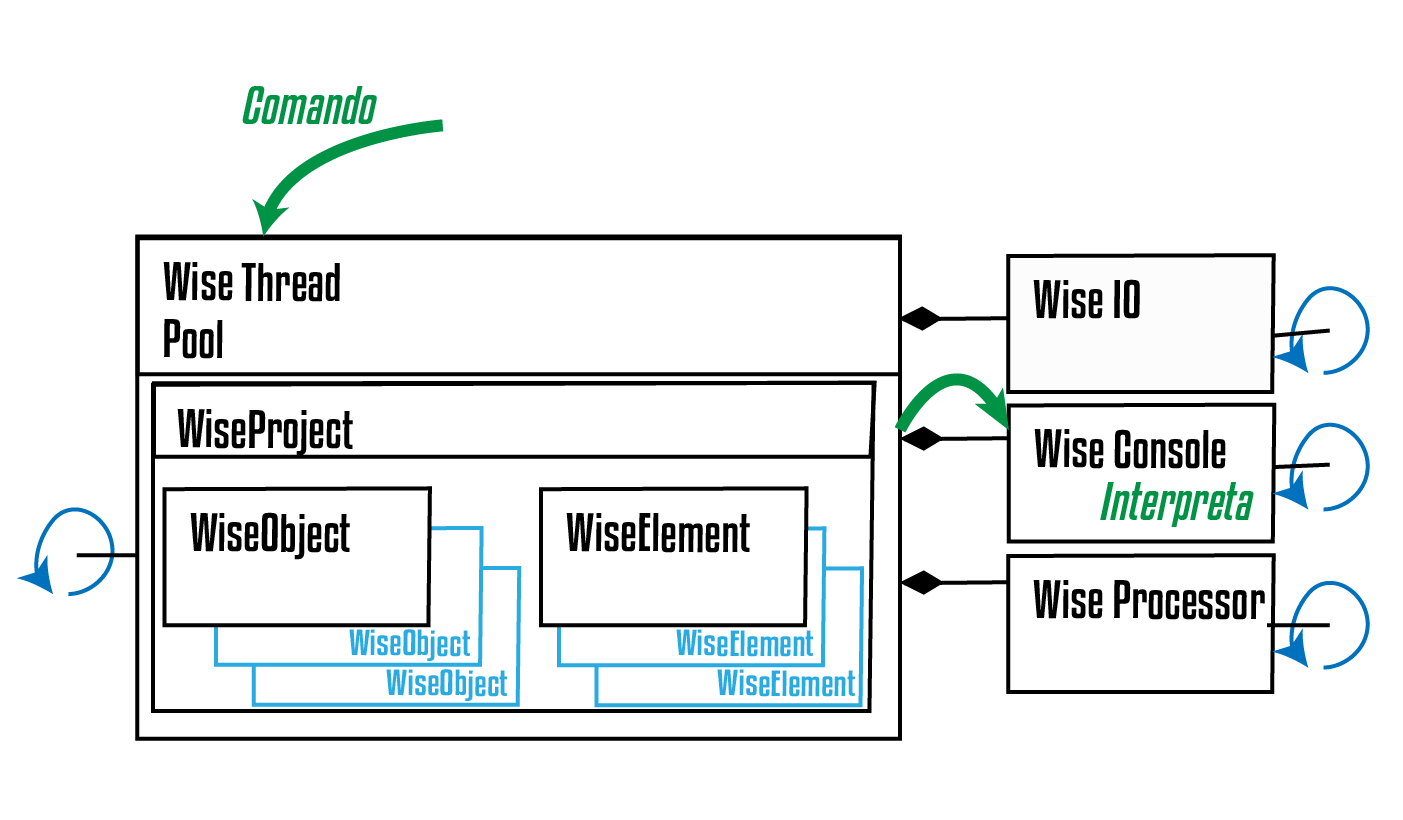
\includegraphics[scale=1]{Figures/WiseThreaPoolCMD.png}
	\caption{Modelo de Threads ao receber uma linha de comando da interface de usuário.}
	\label{fig8:threads}
\end{figure}

Quando se trata de um comando de escrita ou leitura, a thread \textit{WiseIO} é utilizada, ao receber esse tipo de comando o console inteligente irá listar o trabalho no gerenciador de threads \textit{WiseThreadPool}. O gerenciador irá balancear a as requisições entre as threads, em seguida o gerenciador de threads irá aguardar uma mensagem indicando o final da execução do trabalho. Quando um objeto inteligente \textit{WiseObject} é iterado um elemento inteligente é criado na estrutura \textit{Freezer}, ao ser criado o objeto inteligente irá requisitar através de um trabalho inteligente que esse elemento seja armazenado. Portanto a thread \textit{WiseIO} é muito utilizada no ciclo de vida de um elemento inteligente, gerenciando o processo de armazenamento e reconstrução do elemento. É esta estrutura que efetivamente aquece e resfria elementos inteligentes.

\begin{figure}[!htbp]
	\centering
	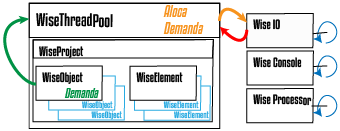
\includegraphics[scale=1]{Figures/WiseThreadPoolHeating.png}
	\caption{Modelo de Threads ao receber um comando de escrita/leitura.}
	\label{fig9:threads}
\end{figure}

Os trabalhos de iteração funcionam da mesma forma que as de leitura ou escrita, entretanto são enviadas a threads \textit{WiseProcessor}. Essas threads não possuem lógicas muito complexas, elas são responsáveis apenas por gerenciar os objetos e chamar os métodos equivalentes, por este motivo os objetos inteligentes e elementos inteligentes possuem métodos abstratos e seguem esses conjuntos de regras, para que uma estrutura que desconheça o seu funcionamento ou suas estruturas internas seja capaz de executar métodos padrões. 

Mesmo com a arquitetura de threads inclusa na ferramenta computacional ainda é possível que ela seja executada em plataformas de thread única, neste caso mais threads inteligentes não farão diferença. Pois apesar dos trabalhos ainda serem dividos em threads diferentes, elas serão executadas no mesmo núcleo de processamento. As threads inteligentes têm um impacto maior nas atividades de escrita e leitura, isto porque o objeto inteligente está divido em várias estruturas menores que são armazenadas e acessadas constantemente, principalmente no caso de uma animação gráfica.

%-------------------------------------------------------------------------------------------%
\section{INTERFACE DE USUÁRIO}\label{sec:userinterface}

Nesta seção apresentam-se detalhes da interface escolhida para facilitar o uso da ferramenta computacional. A interface de usuário foi concebida para permitir o controle de todas as estruturas descritas na Seção~\ref{sec:estrutura} com todos os seus recursos gráficos extraídos. A interface se divide em duas partes principais: Um console, que permite uma interação textual e acesso as mesmas funcionalidades de iteração; E uma janela com elementos gráficos capazes de exibir os resultados gráficos obtidos. 

\begin{figure}[!htbp]
	\centering
	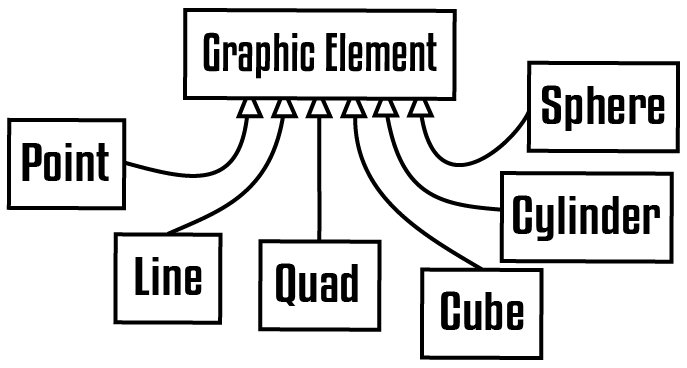
\includegraphics[scale=1]{Figures/GraphicElements}
	\caption{Interface de usuário gráfica.}
	\label{fig10:UI}
\end{figure}

Ambas as estruturas foram construídas para manipular objetos inteligentes e suas estruturas, por isto ambas possuem instâncias do gerenciador de threads inteligentes descritos na Seção~\ref{sec:estrutura}. O console se trata de um  envio direto de mensagens para a thread \textit{WiseConsole}, que é efetivamente o console. Nas próximas seções os diferentes ambientes da ferramenta computacional serão descritos. Cada ambiente representa um projeto \textit{Qt}/\textit{C++} distinto, no projeto do console as bibliotecas gráficas do OpenGl não foram incluídas no processo de compilação, portanto computadores sem grandes recursos gráficos podem executar a mesma lógica de iteração.

%--------------------------------------------------------------------------------%
\subsection{CONSOLE}\label{sec:console}

O ambiente do console consiste em um projeto \textit{Qt}/\textit{C++} sem interface gráfica, ao executar o programa o cabeçalho é impresso e os comandos de entrada são aguardados. O projeto do console foi intitulado \textit{InGU} ou Iterador não-Gráfico Universal, isto porque este projeto apesar de não conter elementos gráficos e exibir os resultados numéricos em tempo de execução é capaz de gerar as estruturas gráficas para visualização futura.

A única  estrutura presente neste projeto é o gerenciador de threads inteligente, isso permite que através de comandos de texto as mesmas estruturas sejam utilizadas.


\begin{figure}[!htbp]
	\centering
	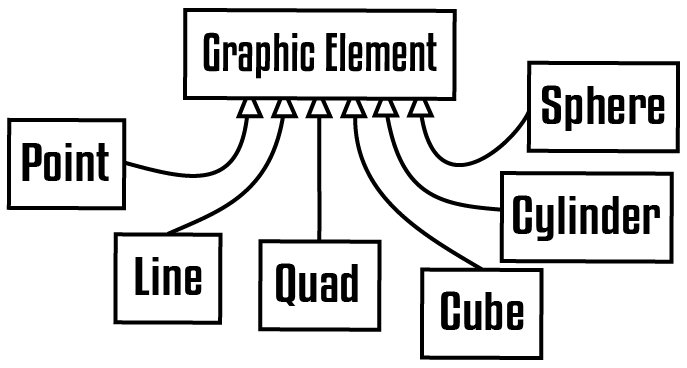
\includegraphics[scale=1]{Figures/GraphicElements}
	\caption{Interface de usuário gráfica.}
	\label{fig10:UI}
\end{figure}

No anexo estão as sequências de instruções necessárias para compilar ambas as partes da ferramenta computacional. Ao ser compilado, um executável InGU contendo o projeto console é gerado, o processo de compilação da ferramenta é multiplataforma, tendo sido testado nos sistemas operacionais \textit{Windows} e \textit{Linux}. Entretanto, recomenda-se a utilização da ferramenta computacional no \textit{Linux}. Ao ser executado, o console corresponde do sistema operacional irá ser aberto com o cabeçalho da ferramenta e aguardará entrada de texto.

IMAGEM CONSOLE

Para executar um comando, basta inserir uma linha de texto e apertar a tecla \textit{Enter}.  Ao capturar a linha de texto, o programa de console irá na verdade redirecionar o comando para a estrutura \textit{WiseThreadPool}, que por sua vez irá alocar uma thread do tipo \textit{WiseConsole} para interpretar a mensagem. Este comportamento é o mesmo apresentado na Seção~\ref{sec:threads}. Uma lista de comandos foi disponibilizada e está acessível através do comando \textit{help}. Ao enviar este comando para o console uma lista com todos as possíveis entradas será exibida. Nas próximas seções estes comandos e suas entradas serão descritos em profundidade.

%--------------------------------------------------------------------------------%
\subsubsection{HELP}\label{sec:help}

O comando de ajuda é o primeiro comando da interface e foi feito para listar todas as entradas possíveis do programa.

\begin{center}
	\begin{tabular}{|c|c|}
		\hline
		\textbf{Linha de Comando} & help \\
		\hline
		\textbf{Entrada} & Nenhuma \\
		\hline
	\end{tabular}
\end{center}

IMAGEM CONSOLE HELP

Ao executar o comando, o usuário receberá uma lista de comandos divididos em escopos específicos. Os escopos foram criados para agrupar comandos por área de atuação, comandos auxiliares, como o comando de ajuda, são os comandos que não alteram as estruturas e exibem informações auxiliares ao usuário.


%--------------------------------------------------------------------------------%
\subsubsection{LER ARQUIVO DE ENTRADA}\label{sec:read_cmds}


O comando de leitura de arquivo de comandos irá receber o endereço de um arquivo local, este arquivo deve conter um comando por linha, um exemplo pode ser encontrado no Anexo~\ref{annex2}. Para este tipo de comando um \textit{WiseJob} contendo a linha de comando e qual a sequência de trabalhos que deve ser executada.

\begin{center}
	\begin{tabular}{|c|c|c|}
		\hline
		\textbf{Linha de Comando} & \multicolumn{2}{c}{read_cmds <file>} \\
		\hline
		\textbf{Entrada} & \textbf{<file>} & Caminho para arquivo contendo sequência de comandos. \\
		\hline
	\end{tabular}
\end{center}

%--------------------------------------------------------------------------------%
\subsubsection{BATERIA DE TESTES}\label{sec:test}

O ciclo principal de testes da ferramente se baseia em verificar a consistência de todas as fábricas e do fluxo principal da ferramenta computacional, exceto detalhes gráficos e do processo de iteração. Ao executar a bateria de testes todos os elementos inteligentes \textit{WiseElement} disponíveis e todos os objetos inteligentes \textit{WiseObject} serão testados individualmente. Cada uma destas estruturas irá ser construída, então salva em em um arquivo externo. Em seguida o arquivo é reconstruído e a estrutura resultante comparada com a primeira, caso sejam iguais o resultado de sucesso é armazenado.

Estes testes foram utilizados principalmente no momento do desenvolvimento da ferramenta e garantem que as fábricas de elementos e objetos inteligentes estão funcionando corretamente. Futuramente, caso novas estruturas sejam incluídas, estes testes garantem que todas as classes do projeto foram projetadas corretamente, com isso todas as estruturas que são carregadas pela ferramenta não perdem informação ao serem armazenadas e recuperadas, processo recorrente na ferramenta computacional.

\begin{center}
	\begin{tabular}{|c|c|}
		\hline
		\textbf{Linha de Comando} & test \\
		\hline
		\textbf{Entrada} & Nenhuma \\
		\hline
	\end{tabular}
\end{center}

%--------------------------------------------------------------------------------%
\subsubsection{LISTA DE TESTES}\label{sec:test list}



\begin{center}
	\begin{tabular}{|c|c|}
		\hline
		\textbf{Linha de Comando} & test list \\
		\hline
		\textbf{Entrada} & Nenhuma \\
		\hline
	\end{tabular}
\end{center}

%--------------------------------------------------------------------------------%
\subsection{JANELA}\label{sec:janela}

%-------------------------------------------------------------------------------------------%
\chapter{RESULTADOS NUMÉRICOS E DISCUSSÕES}

\begin{itemize}
	\item \textcolor{red}{IGOR: já fiz uma primeira revisão deste capítulo e indico em vermelho o que deve fazer para melhorar este capítulo. Tudo que acrescentar ou mudar coloque em azul.}
	\item \textcolor{red}{IGOR: não está aparecendo a numeração das Figuras no caption. Algo de errado está acontecendo no modelo que está utilizando.}
	\item \textcolor{red}{IGOR: está errada a citação do trabalho do método de Duan e Zamir (1995), não é a citação que colocou \cite{Duan}.}\textcolor{green}{\textbf{OK}}
\end{itemize}

Nesta seção, apresentam-se resultados obtidos com a implementação computacional e simulação do modelo matemático de Duan e Zamir~\cite{Duan1992}. As simulações realizadas aqui tratam da propagação de uma onda harmônica simples ao longo de uma árvore, onde reflexões de onda modificam a amplitude da onda de pressão enquanto ela avança. A escolha de uma onda harmônica simples neste estudo possibilita investigar os efeitos da frequência, fluido viscoso e viscoelasticidade da parede do segmento de vaso.

Considerou-se neste estudo um modelo de árvore arterial canina como ilustrado na Figura~\ref{fig:arvore-canina}. As propriedades dos segmentos foram escolhidas oriundas dos dados de Fung~\cite{Fung} e são descritas na Tabela~\ref{tab1:proprerty}. 

\begin{figure}[!htbp]
	\centering
	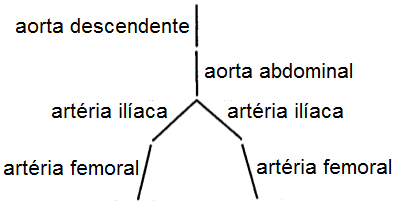
\includegraphics[scale=0.8]{Figures/tree_canine.png}
	\caption{Representação do modelo de árvore arterial canina (figura adaptada de~\cite{Duan}).}
	\label{fig:arvore-canina}
\end{figure}

\begin{table}[!htbp]
	\caption{Propriedades dos segmentos do modelo de árvore arterial~\cite{Duan,Fung}}
	\centering{}
	\begin{tabular}{|c||c|c|c|c|c|}
		\hline 
		Artéria	& Comprimento & Densidade & Viscosidade  & Diâmetro & Módulo de  \\ 
		& ($cm$) & $\rho$ ($g/cm^3$) & $\mu_0$ ($g/cm s$) & ($cm$) & Young ($dyn/cm^2$) \\ 
		\hline
		\hline 
		Aorta & 25 & $0,960$ & 0,0385 & 1,3 &4,8 $\times 10^6$ \\ 
		Descendente &  & &  & & \\ 
		\hline 
		Aorta & 11 & $1,134$ & 0,0449 & 0,9 & 1,0 $\times 10^7$ \\
		Abdominal &  & &  & &  \\ 
		\hline 
		Ilíaca & 12 & $1,172$ & 0,0472 & 0,6 & 1,0 $\times 10^7$\\ 
		\hline 
		Femoral & 10 & $1,235$ & 0,0494 & 0,4 & 1,0 $\times 10^7$\\ 
		\hline 
	\end{tabular} 
	\label{tab1:proprerty}
\end{table}

Nas simulações aqui realizadas, calculou-se a distribuição de amplitude de pressão ao longo da árvore arterial (Figura~\ref{fig:arvore-canina}). Os resultados foram obtidos para quatro diferentes frequên\-cias e três diferentes cenários de escoamento/segmento: (i) escoamento viscoso em segmento puramente elástico (cenário 1 da Seção~\ref{sec:cenario}), (ii) escoamento invíscido em segmento viscoelástico (cenário 2) e (iii) escoamento viscoso em segmento viscoelástico (cenário 3). 

Os resultados obtidos nas simulações são mostrados nas Figuras~\ref{fig3a:arterial-tree}, \ref{fig3b:arterial-tree}, \ref{fig4a:arterial-tree}, \ref{fig4b:arterial-tree}, \ref{fig5a:arterial-tree} envolvendo a amplitude da pressão ao longo do modelo de árvore arterial. Nestas figuras, o comprimento de cada segmento arterial foi dimensionado para 1,0, de modo que o comprimento adimensional total da árvore é 4,0. O comprimento real é 58 cm. A amplitude da pressão também foi escalada pela pressão de entrada $P_o$, e os resultados finais são portanto mostrados em termos de amplitude de pressão adimensional $|P|$ versus a distância adimensional $X$ do início da árvore.

Nas Figuras~\ref{fig3a:arterial-tree} e \ref{fig3b:arterial-tree}, o efeito da viscosidade do fluido é examinado separadamente conside\-ran\-do-se o escoamento em segmentos puramente elásticos com quatro valores diferentes de viscosidade do fluido, ou seja, $\mu = 0$; $0,5 \mu_0$; $1,0 \mu_0$ e $1,5 \mu_0$, onde $\mu_0$ é o valor base da viscosidade da Tabela~\ref{tab1:proprerty}. Observa-se que o efeito da viscosidade do fluido é reduzir o aumento global na amplitude da onda de pressão causada pelas reflexões das ondas à medida que a onda se desloca na direção à jusante. Além disso, modera os picos locais na distribuição de pressão.

\begin{figure}[!htbp]
	\centering
	(a) \\
		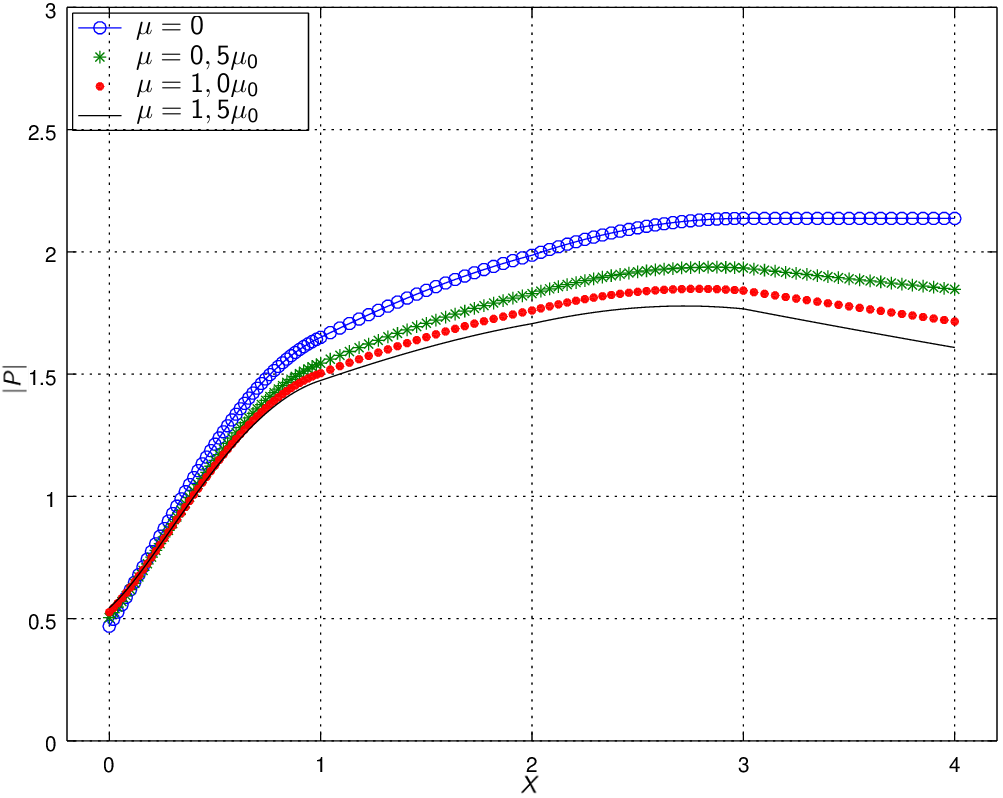
\includegraphics[scale=0.7]{figure3-result-new/fig3_P_f3_65_visc_new2.png}\\
	(b)\\
	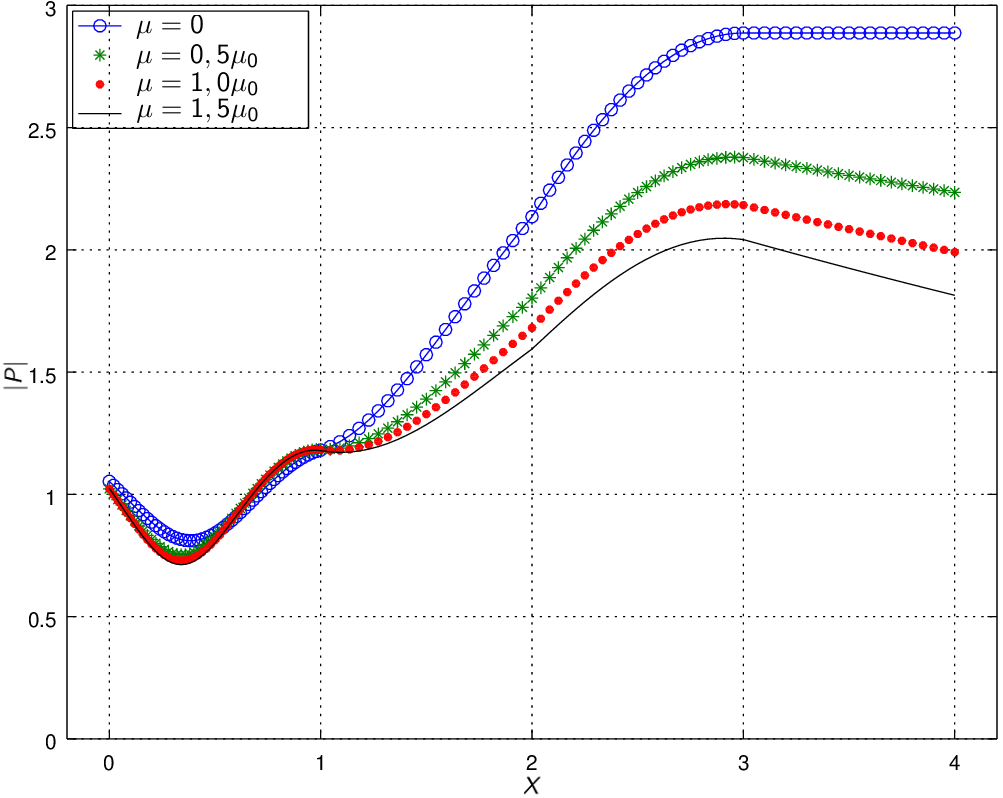
\includegraphics[scale=0.7]{figure3-result-new/fig3_P_f7_30_visc_new2.png}\\
	\caption{Amplitude da pressão $|P|$ ao longo da árvore arterial considerando diferentes viscosidade do fluido $\mu$ e frequências: (a) $f$ = 3,65 Hz, (b)  $f$ = 7,30 Hz. }
	\label{fig3a:arterial-tree}%
\end{figure}

\begin{figure}[!htbp]
	\centering
	(a) $f$ = 10,95 Hz\\
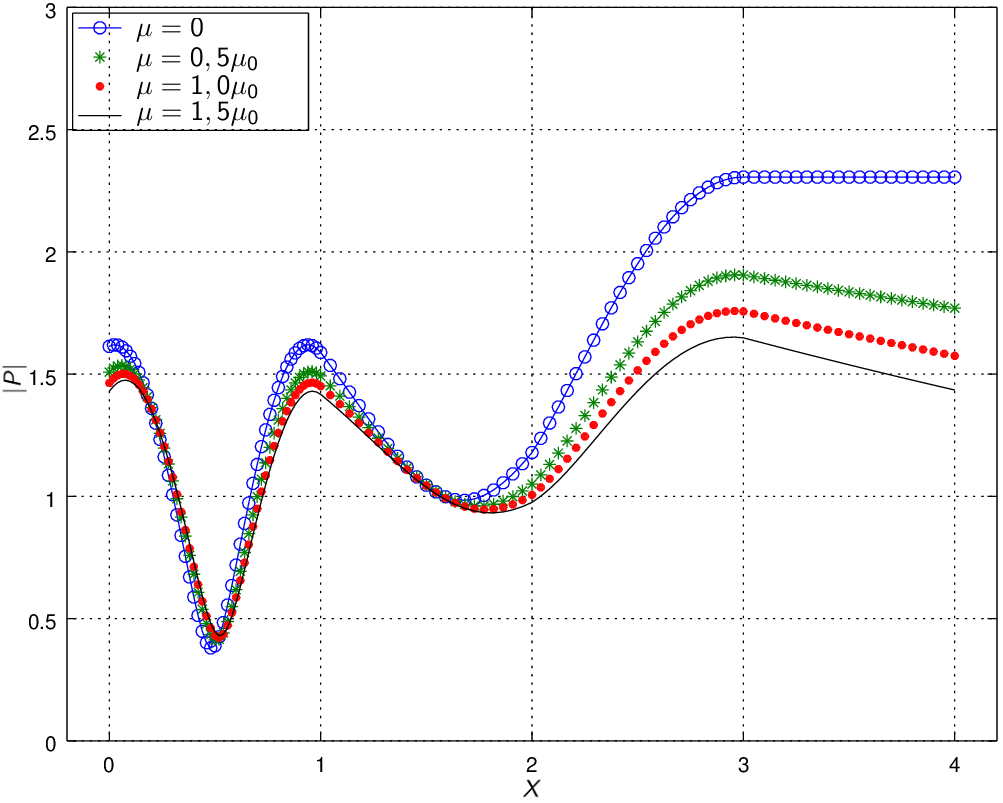
\includegraphics[scale=0.7]{figure3-result-new/fig3_P_f10_95_visc_new2.png}\\
	(b) $f$ = 14,60 Hz\\
	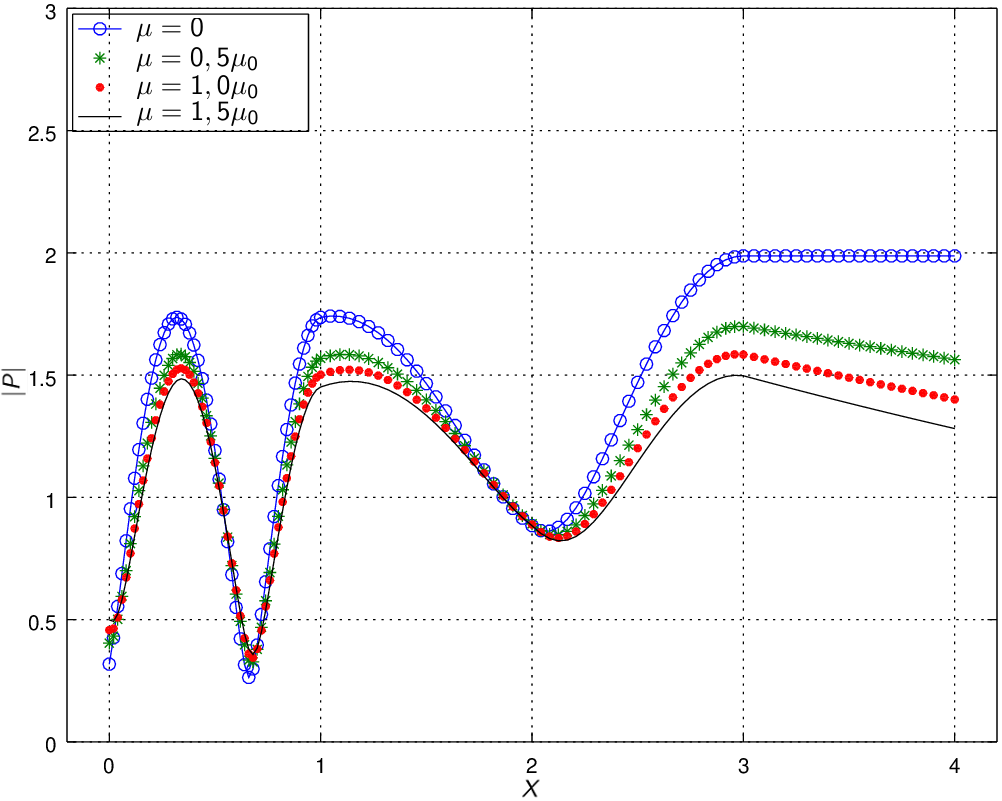
\includegraphics[scale=0.7]{figure3-result-new/fig3_P_f14_60_visc_new2.png}\\
	\caption{Amplitude da pressão $|P|$ ao longo da árvore arterial considerando diferentes viscosidade do fluido $\mu$ e frequências: (a) $f$ = 10,95 Hz, (b)  $f$ = 14,60 Hz. }
	\label{fig3b:arterial-tree}%
\end{figure}

Nas Figuras~\ref{fig4a:arterial-tree}, \ref{fig4b:arterial-tree}, o efeito da viscoelasticidade da parede do segmento de vaso é considerado separadamente considerando-se o escoamento invíscido e tomando-se quatro valores diferentes da viscoelasticidade da parede do segmento. O modelo viscoelástico proposto utilizado para fins destes cálculos é apresentado no cenário 2 da Seção~\ref{sec:cenario}, no qual a viscoelasticidade da parede do vaso é representada por um módulo de Young complexo. Estas figuras mostram os resultados para $\phi_0$ = $0^o$, $4^o$, $8^o$ e $12^o$. Quando $\phi_0$ = $0^o$ tem-se um valor representando uma parede puramente elástica e para $\phi_0> 0$ tem-se a representação da viscoelasticidade. Nota-se a partir destas figuras que o efeito da viscoelasticidade, como o da viscosidade do fluido, é amortecer o aumento global da amplitude da onda de pressão causada pelas reflexões das ondas à medida que a onda se desloca na direção à jusante, bem como moderar os picos locais na distribuição de pressão. 

\begin{figure}[!htbp]
	\centering
	(a) \\
	\includegraphics[scale=0.7]{figure4-result-new/Fig4_P_f3_65_visco_new2.png}\\
	(b)\\
	\includegraphics[scale=0.7]{figure4-result-new/Fig4_P_f7_30_visco_new2.png}\\
	\caption{Amplitude da pressão $|P|$ ao longo da árvore arterial considerando diferentes valores de viscoelasticidade $\phi_0$ e frequências: (a) $f$ = 3,65 Hz, (b)  $f$ = 7,30 Hz. }
	\label{fig4a:arterial-tree}%
\end{figure}

\begin{figure}[!htbp]
	\centering
	(a) $f$ = 10,95 Hz\\
	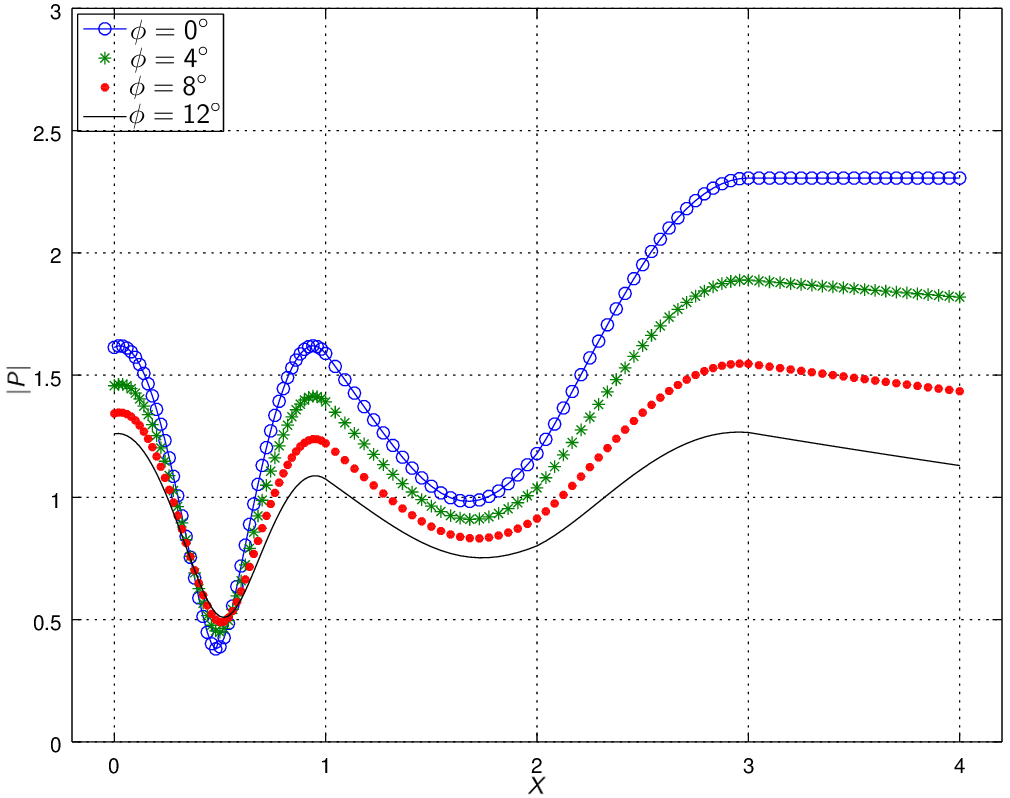
\includegraphics[scale=0.7]{figure4-result-new/fig4_P_f10_95_visco_new2.png}\\
	(b) $f$ = 14,60 Hz\\
	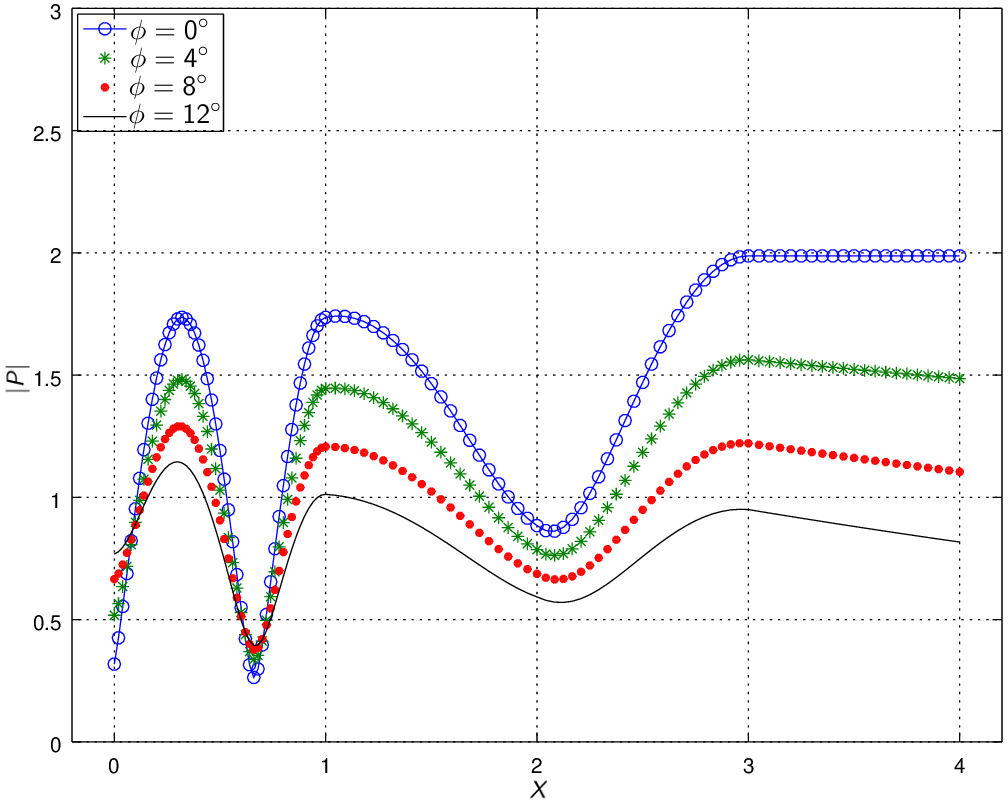
\includegraphics[scale=0.7]{figure4-result-new/fig4_P_f14_60_visco_new2.png}\\
	\caption{Amplitude da pressão $|P|$ ao longo da árvore arterial considerando diferentes valores de viscoelasticidade $\phi_0$ e frequências: (a) $f$ = 10,95 Hz, (b) $f$ = 14,60 Hz.}
	\label{fig4b:arterial-tree}%
\end{figure}

A Figura \ref{fig:impedance1} apresenta o comportamento da impedância de entrada $|Z|$ em função da frequência $f$, que está coerente com dados experimentais ~\cite{Nichols2011} da aorta. Na Figura \ref{fig:impedance1}a, nota-se que, quando se considera a viscosidade ($\mu \neq 0$) na simulação do método, isso afeta a impedância de entrada para frequências que se aproximam de 0 Hz e atenua o pico que surge na curva entre 10 Hz e 12,5 Hz. Além disso, neste intervalo de frequência, observa-se o aparecimento do pico mencionado em uma frequência ligeiramente menor com o aumento de $mu$.

No tocante ao impacto da viscoelasticidade da parede na impedância de entrada, o aumento do parâmetro $\phi$ reduz o pico que aparece na curva de impedância entre 10 Hz e 12,5 Hz como pode ser visto na Figura \ref{fig:impedance1}b. Diferente da Figura \ref{fig:impedance1}a, o pico destacado surge na mesma frequência independente do $\phi$.

\begin{figure}[!htbp]
	\centering
	(a) \\
	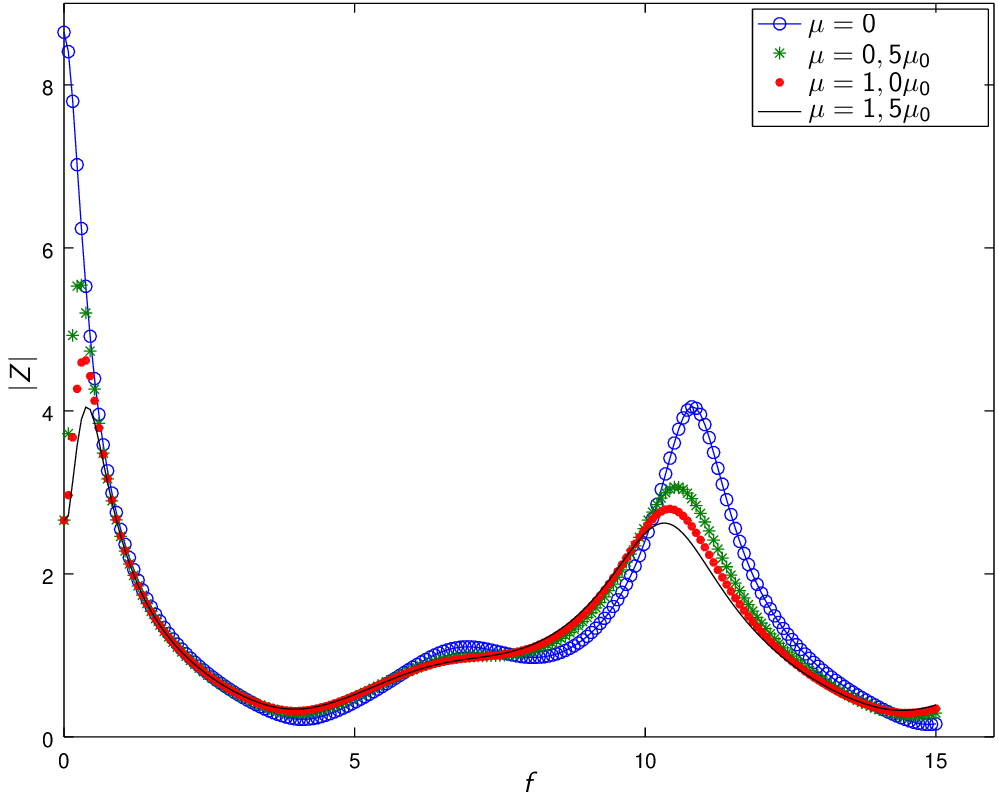
\includegraphics[scale=0.7]{figure-result-impedance/fig_viscosity_impedance_new.png}\\
		(b) \\
	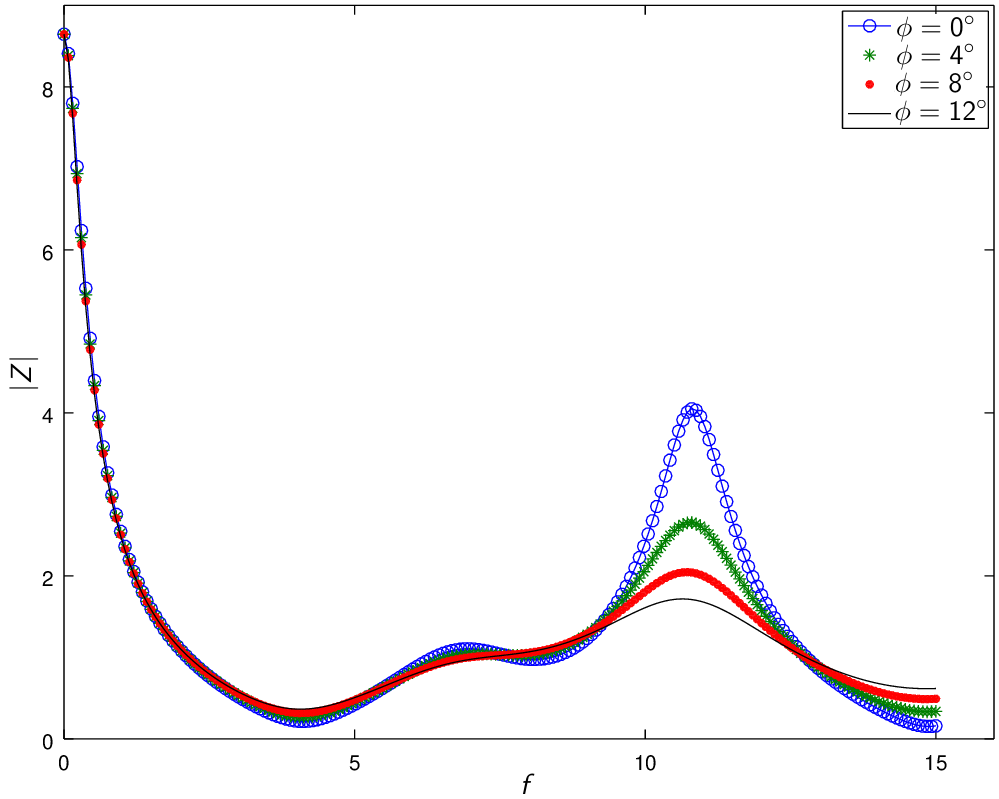
\includegraphics[scale=0.7]{figure-result-impedance/fig_viscoelasticity_impedance_new.png}
	\caption{Amplitude da impedância de entrada $|Z|$ em função da frequência $f$: (a) efeito da viscosidade (b) impacto da viscoelasticidade.}
	\label{fig:impedance1}%
\end{figure}

%\newpage
Os efeitos combinados da viscosidade do fluido e viscoelasticidade da parede do vaso na amplitude de pressão $P$ e impedância de entrada $Z$ são mostrados nas Figuras \ref{fig5a:arterial-tree} e \ref{fig5b:arterial-tree}. Os valores $\mu = 1,0 \mu_0$ e $\phi_0 = 8^o$ foram utilizados para este propósito, para serem comparados com os mesmos valores dos resultados anteriores. A observação mais importante a ser feita é que os dois efeitos, quando combinados, não se somam. Por outro lado, combinam-se de uma maneira não linear que não é prontamente previsível.

\begin{figure}[!htbp]
	\centering
	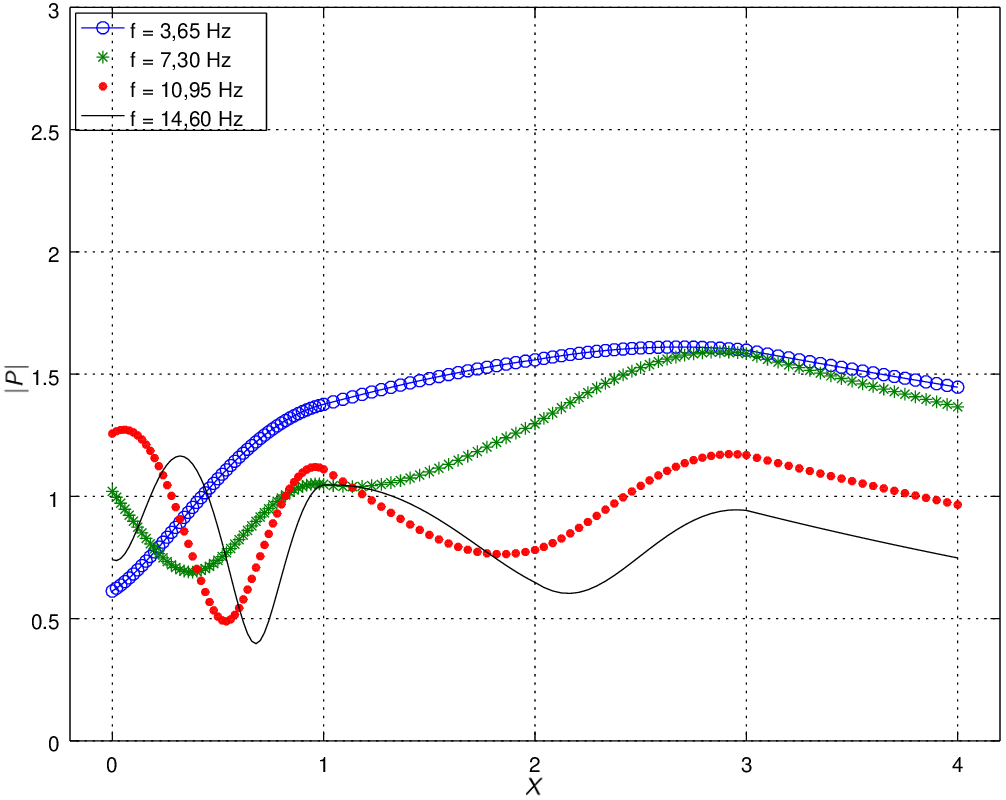
\includegraphics[scale=0.7]{figure5-result-new/Fig5_P_visc1_phi8_new2.png}
	\caption{Amplitude da pressão $|P|$ ao longo da árvore arterial $X$ considerando viscosidade $\mu = 1,0 \mu_0$, viscoelasticidade $\phi_0 = 8^{\circ}$.}
	\label{fig5a:arterial-tree}%
\end{figure}

\begin{figure}[!htbp]
	\centering
	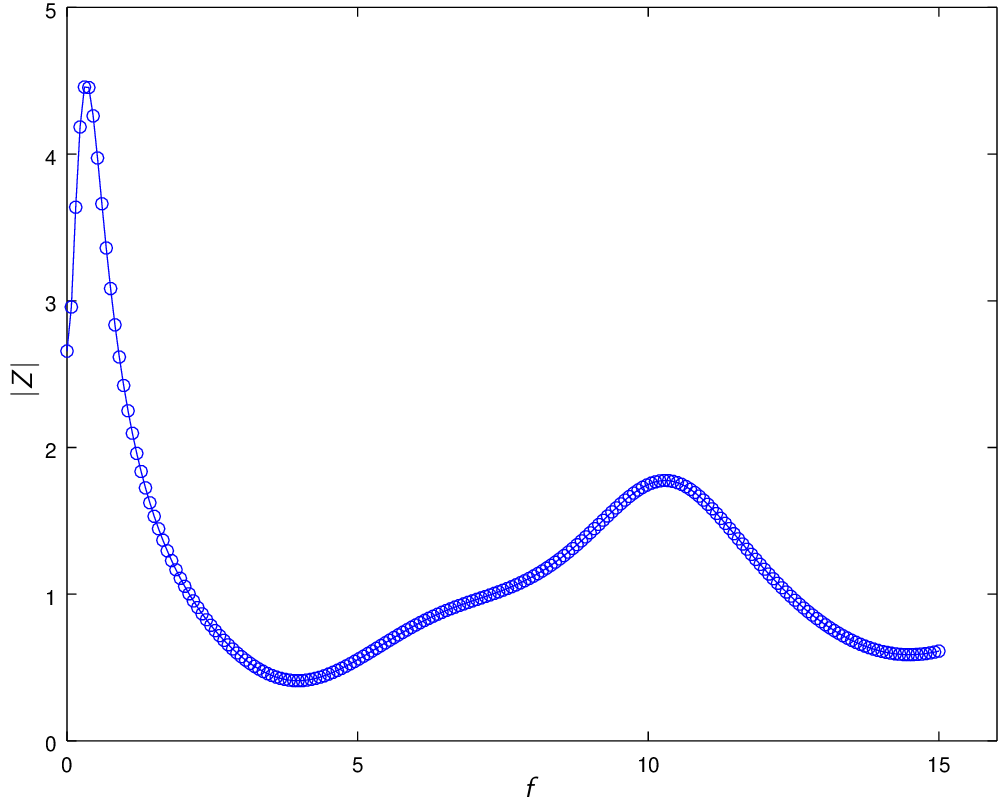
\includegraphics[scale=0.7]{figure-result-impedance/fig_viscosidade1_viscoelasticity8_impedance_new.png}
	\caption{Impedância de entrada $|Z|$ em função da frequência $f$ considerando viscosidade $\mu = 1,0 \mu_0$, viscoelasticidade $\phi_0 = 8^{\circ}$.}
	\label{fig5b:arterial-tree}%
\end{figure}

%-----------------------------------------------------------------------------------------%
\chapter{CONCLUSÕES E TRABALHOS FUTUROS}
\textcolor{red}{IGOR: já fiz uma primeira revisão deste capítulo e indico em vermelho o que deve fazer para melhorar este capítulo. Tudo que acrescentar ou mudar coloque em azul.}
\textcolor{blue}{XXXXXXXXXXXXX}.

Em relação a hemodinâmica, os resultados obtidos neste trabalho estão de acordo com aqueles obtidos por Duan e Zamir\textcolor{blue}{ \cite{Duan1992} } considerando a propagação de uma onda harmônica simples nos três cenários abordados nas simulações. 

Em destaque, visando contribuir na investigação do método desenvolvido por por Duan e Zamir, curvas de impedância de entrada do modelo de árvore canina aqui considerada foram apresentadas. Estas curvas apresentam comportamento que pode ser observado em dados experimentais.

A realização deste trabalho resultou no desenvolvimento de uma nova ferramenta computacional descrita no Capítulo~\ref{sec:modelagem}, que permite a simulação de escoamento sanguíneo pulsátil em modelos de árvores arteriais no contexto de Duan e Zamir. 

\textcolor{red}{IGOR: escreva um parágrafo destacando propriedades/características e potencialidades da sua ferramenta computacional. Talvez você poderá recuperar ou utilizar algo do parágrafo abaixo.}

\textcolor{red}{A ferramenta simula e analisa modelos de árvores arteriais. Ela pode ser utilizada nos sistemas Operacionais: Windows e o Ubuntu (Unix). Os modelos podem ter sua análise e gráficos gerados automaticamente através dos comandos da ferramenta computacional. O código possibilita o processamento concorrente de diversos modelos em um mesmo ambiente. Cada uma destas contribuições resultou numa ferramenta robusta,  ferramenta esta que além de analisar corretamente as variações de fluxo e pressão através de um modelo de árvore arterial, possibilita que as simulações sejam facilmente ajustadas e analisadas, com ou sem interface gráfica.}

\textcolor{red}{IGOR: o parágrafo acima descreve a ferramenta descrita no Capítulo 3? Este parágrafo representa a descrição da ferramenta.}

Como trabalhos futuros, destacam-se:
\begin{itemize}
    \item Analisar hemodinamicamente modelos de árvores gerados no contexto do método CCO (\emph{Constrained Constructive Optimization}) \cite{Karch1999,Queiroz2013,Queiroz2015,Brito2017};
    \item Investigar a influência da escolha parâmetros na resposta do método, tais como: módulo de Young e espessura do vaso;
    \item \textcolor{red} {IGOR: descreva algo que poderia ser interessante agregar na ferramenta, pode ser mais de uma coisa (coloque em item)}.
\end{itemize}

\begin{appendices}
	%-----------------------------------------------------------------------------------------%
	\chapter{PROCESSO DE COMPILAÇÃO}\label{annex1}
	
	
	%-----------------------------------------------------------------------------------------%
	\chapter{FORMATO DE ARQUIVO DE COMANDOS}\label{annex2}
	
	
	
	
\end{appendices}

\bibliographystyle{abntex2-alf}
\bibliography{referencias}


\end{document}
